\documentclass[twoside]{book}

% Packages required by doxygen
\usepackage{fixltx2e}
\usepackage{calc}
\usepackage{doxygen}
\usepackage[export]{adjustbox} % also loads graphicx
\usepackage{graphicx}
\usepackage[utf8]{inputenc}
\usepackage{makeidx}
\usepackage{multicol}
\usepackage{multirow}
\PassOptionsToPackage{warn}{textcomp}
\usepackage{textcomp}
\usepackage[nointegrals]{wasysym}
\usepackage[table]{xcolor}

% Font selection
\usepackage[T1]{fontenc}
\usepackage[scaled=.90]{helvet}
\usepackage{courier}
\usepackage{amssymb}
\usepackage{sectsty}
\renewcommand{\familydefault}{\sfdefault}
\allsectionsfont{%
  \fontseries{bc}\selectfont%
  \color{darkgray}%
}
\renewcommand{\DoxyLabelFont}{%
  \fontseries{bc}\selectfont%
  \color{darkgray}%
}
\newcommand{\+}{\discretionary{\mbox{\scriptsize$\hookleftarrow$}}{}{}}

% Page & text layout
\usepackage{geometry}
\geometry{%
  a4paper,%
  top=2.5cm,%
  bottom=2.5cm,%
  left=2.5cm,%
  right=2.5cm%
}
\tolerance=750
\hfuzz=15pt
\hbadness=750
\setlength{\emergencystretch}{15pt}
\setlength{\parindent}{0cm}
\setlength{\parskip}{3ex plus 2ex minus 2ex}
\makeatletter
\renewcommand{\paragraph}{%
  \@startsection{paragraph}{4}{0ex}{-1.0ex}{1.0ex}{%
    \normalfont\normalsize\bfseries\SS@parafont%
  }%
}
\renewcommand{\subparagraph}{%
  \@startsection{subparagraph}{5}{0ex}{-1.0ex}{1.0ex}{%
    \normalfont\normalsize\bfseries\SS@subparafont%
  }%
}
\makeatother

% Headers & footers
\usepackage{fancyhdr}
\pagestyle{fancyplain}
\fancyhead[LE]{\fancyplain{}{\bfseries\thepage}}
\fancyhead[CE]{\fancyplain{}{}}
\fancyhead[RE]{\fancyplain{}{\bfseries\leftmark}}
\fancyhead[LO]{\fancyplain{}{\bfseries\rightmark}}
\fancyhead[CO]{\fancyplain{}{}}
\fancyhead[RO]{\fancyplain{}{\bfseries\thepage}}
\fancyfoot[LE]{\fancyplain{}{}}
\fancyfoot[CE]{\fancyplain{}{}}
\fancyfoot[RE]{\fancyplain{}{\bfseries\scriptsize Generated by Doxygen }}
\fancyfoot[LO]{\fancyplain{}{\bfseries\scriptsize Generated by Doxygen }}
\fancyfoot[CO]{\fancyplain{}{}}
\fancyfoot[RO]{\fancyplain{}{}}
\renewcommand{\footrulewidth}{0.4pt}
\renewcommand{\chaptermark}[1]{%
  \markboth{#1}{}%
}
\renewcommand{\sectionmark}[1]{%
  \markright{\thesection\ #1}%
}

% Indices & bibliography
\usepackage{natbib}
\usepackage[titles]{tocloft}
\setcounter{tocdepth}{3}
\setcounter{secnumdepth}{5}
\makeindex

% Hyperlinks (required, but should be loaded last)
\usepackage{ifpdf}
\ifpdf
  \usepackage[pdftex,pagebackref=true]{hyperref}
\else
  \usepackage[ps2pdf,pagebackref=true]{hyperref}
\fi
\hypersetup{%
  colorlinks=true,%
  linkcolor=blue,%
  citecolor=blue,%
  unicode%
}

% Custom commands
\newcommand{\clearemptydoublepage}{%
  \newpage{\pagestyle{empty}\cleardoublepage}%
}

\usepackage{caption}
\captionsetup{labelsep=space,justification=centering,font={bf},singlelinecheck=off,skip=4pt,position=top}

%===== C O N T E N T S =====

\begin{document}

% Titlepage & ToC
\hypersetup{pageanchor=false,
             bookmarksnumbered=true,
             pdfencoding=unicode
            }
\pagenumbering{alph}
\begin{titlepage}
\vspace*{7cm}
\begin{center}%
{\Large P2 }\\
\vspace*{1cm}
{\large Generated by Doxygen 1.8.14}\\
\end{center}
\end{titlepage}
\clearemptydoublepage
\pagenumbering{roman}
\tableofcontents
\clearemptydoublepage
\pagenumbering{arabic}
\hypersetup{pageanchor=true}

%--- Begin generated contents ---
\chapter{Hierarchical Index}
\section{Class Hierarchy}
This inheritance list is sorted roughly, but not completely, alphabetically\+:\begin{DoxyCompactList}
\item \contentsline{section}{Customer\+Address}{\pageref{class_customer_address}}{}
\begin{DoxyCompactList}
\item \contentsline{section}{Customer\+List}{\pageref{class_customer_list}}{}
\end{DoxyCompactList}
\item \contentsline{section}{Database\+Manager}{\pageref{class_database_manager}}{}
\item Q\+Dialog\begin{DoxyCompactList}
\item \contentsline{section}{customer\+Listing}{\pageref{classcustomer_listing}}{}
\end{DoxyCompactList}
\item Q\+Main\+Window\begin{DoxyCompactList}
\item \contentsline{section}{Main\+Window}{\pageref{class_main_window}}{}
\end{DoxyCompactList}
\item \contentsline{section}{Services}{\pageref{class_services}}{}
\item \contentsline{section}{Ui\+\_\+customer\+Listing}{\pageref{class_ui__customer_listing}}{}
\begin{DoxyCompactList}
\item \contentsline{section}{Ui\+:\+:customer\+Listing}{\pageref{class_ui_1_1customer_listing}}{}
\end{DoxyCompactList}
\item \contentsline{section}{Ui\+\_\+\+Main\+Window}{\pageref{class_ui___main_window}}{}
\begin{DoxyCompactList}
\item \contentsline{section}{Ui\+:\+:Main\+Window}{\pageref{class_ui_1_1_main_window}}{}
\end{DoxyCompactList}
\end{DoxyCompactList}

\chapter{Class Index}
\section{Class List}
Here are the classes, structs, unions and interfaces with brief descriptions\+:\begin{DoxyCompactList}
\item\contentsline{section}{\mbox{\hyperlink{class_customer_address}{Customer\+Address}} }{\pageref{class_customer_address}}{}
\item\contentsline{section}{\mbox{\hyperlink{class_customer_list}{Customer\+List}} }{\pageref{class_customer_list}}{}
\item\contentsline{section}{\mbox{\hyperlink{class_ui_1_1customer_listing}{Ui\+::customer\+Listing}} }{\pageref{class_ui_1_1customer_listing}}{}
\item\contentsline{section}{\mbox{\hyperlink{classcustomer_listing}{customer\+Listing}} }{\pageref{classcustomer_listing}}{}
\item\contentsline{section}{\mbox{\hyperlink{class_database_manager}{Database\+Manager}} }{\pageref{class_database_manager}}{}
\item\contentsline{section}{\mbox{\hyperlink{class_main_window}{Main\+Window}} }{\pageref{class_main_window}}{}
\item\contentsline{section}{\mbox{\hyperlink{class_ui_1_1_main_window}{Ui\+::\+Main\+Window}} }{\pageref{class_ui_1_1_main_window}}{}
\item\contentsline{section}{\mbox{\hyperlink{class_services}{Services}} }{\pageref{class_services}}{}
\item\contentsline{section}{\mbox{\hyperlink{class_ui__customer_listing}{Ui\+\_\+customer\+Listing}} }{\pageref{class_ui__customer_listing}}{}
\item\contentsline{section}{\mbox{\hyperlink{class_ui___main_window}{Ui\+\_\+\+Main\+Window}} }{\pageref{class_ui___main_window}}{}
\end{DoxyCompactList}

\chapter{File Index}
\section{File List}
Here is a list of all documented files with brief descriptions\+:\begin{DoxyCompactList}
\item\contentsline{section}{C\+:/\+Users/\+Kevin/\+Documents/\+Git\+Hub/i\+Cyber\+Security/project2/\mbox{\hyperlink{constants_8h}{constants.\+h}} \\*Links the database file to the program }{\pageref{constants_8h}}{}
\item\contentsline{section}{C\+:/\+Users/\+Kevin/\+Documents/\+Git\+Hub/i\+Cyber\+Security/project2/\mbox{\hyperlink{customeraddress_8h}{customeraddress.\+h}} \\*Contains data in regard to customer addresses }{\pageref{customeraddress_8h}}{}
\item\contentsline{section}{C\+:/\+Users/\+Kevin/\+Documents/\+Git\+Hub/i\+Cyber\+Security/project2/\mbox{\hyperlink{customerlist_8h}{customerlist.\+h}} \\*Contains data in regard to customers }{\pageref{customerlist_8h}}{}
\item\contentsline{section}{C\+:/\+Users/\+Kevin/\+Documents/\+Git\+Hub/i\+Cyber\+Security/project2/\mbox{\hyperlink{customerlisting_8h}{customerlisting.\+h}} \\*Contains interface options for the customer listing page }{\pageref{customerlisting_8h}}{}
\item\contentsline{section}{C\+:/\+Users/\+Kevin/\+Documents/\+Git\+Hub/i\+Cyber\+Security/project2/\mbox{\hyperlink{databasemanager_8h}{databasemanager.\+h}} \\*Handles information sent to and read from a database file }{\pageref{databasemanager_8h}}{}
\item\contentsline{section}{C\+:/\+Users/\+Kevin/\+Documents/\+Git\+Hub/i\+Cyber\+Security/project2/\mbox{\hyperlink{mainwindow_8h}{mainwindow.\+h}} \\*Manages the user interface of the program }{\pageref{mainwindow_8h}}{}
\item\contentsline{section}{C\+:/\+Users/\+Kevin/\+Documents/\+Git\+Hub/i\+Cyber\+Security/project2/\mbox{\hyperlink{services_8h}{services.\+h}} \\*Contains data in regard to company services }{\pageref{services_8h}}{}
\item\contentsline{section}{C\+:/\+Users/\+Kevin/\+Documents/\+Git\+Hub/i\+Cyber\+Security/project2/{\bfseries ui\+\_\+customerlisting.\+h} }{\pageref{ui__customerlisting_8h}}{}
\item\contentsline{section}{C\+:/\+Users/\+Kevin/\+Documents/\+Git\+Hub/i\+Cyber\+Security/project2/{\bfseries ui\+\_\+mainwindow.\+h} }{\pageref{ui__mainwindow_8h}}{}
\end{DoxyCompactList}

\chapter{Class Documentation}
\hypertarget{class_customer_address}{}\section{Customer\+Address Class Reference}
\label{class_customer_address}\index{Customer\+Address@{Customer\+Address}}


Holds property values for a singular customer address.  




{\ttfamily \#include $<$customeraddress.\+h$>$}

Inheritance diagram for Customer\+Address\+:\begin{figure}[H]
\begin{center}
\leavevmode
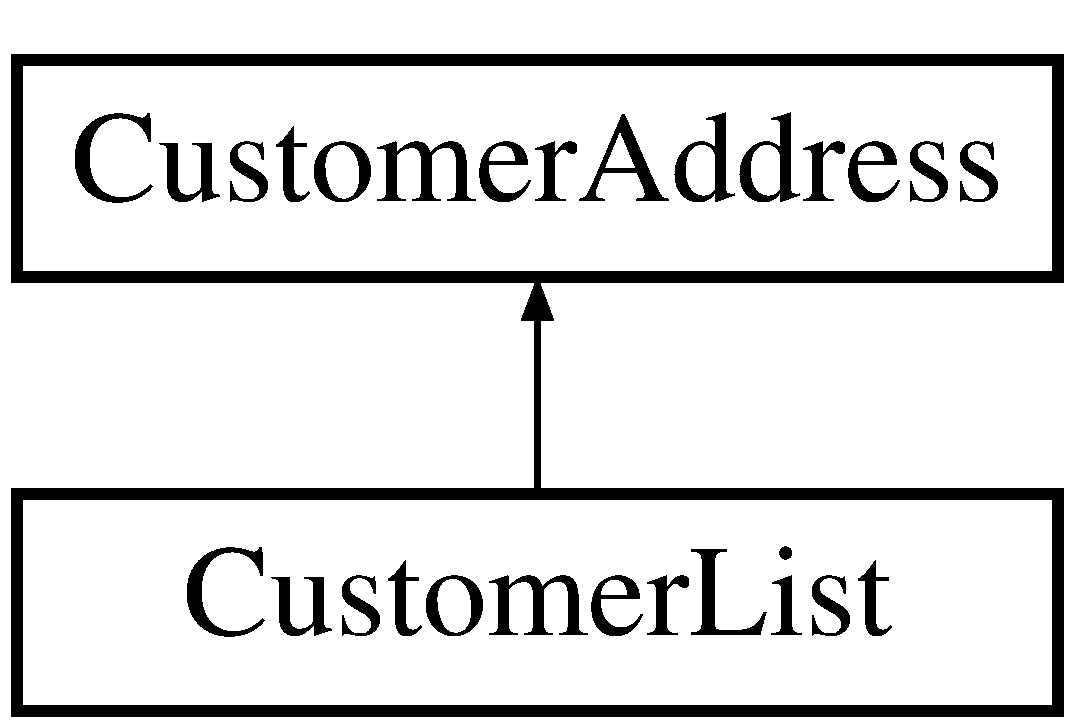
\includegraphics[height=2.000000cm]{class_customer_address}
\end{center}
\end{figure}
\subsection*{Public Member Functions}
\begin{DoxyCompactItemize}
\item 
\mbox{\Hypertarget{class_customer_address_a42b4b2cf860db0f31626f97bf55ca1a3}\label{class_customer_address_a42b4b2cf860db0f31626f97bf55ca1a3}} 
{\bfseries Customer\+Address} (Q\+String, Q\+String, Q\+String, int)
\item 
\mbox{\Hypertarget{class_customer_address_a75d3fb31489664f2f524df57dce4b987}\label{class_customer_address_a75d3fb31489664f2f524df57dce4b987}} 
Q\+String {\bfseries Get\+Street} () const
\item 
\mbox{\Hypertarget{class_customer_address_ac7ea47e415c0c51577fa2ae4f8780312}\label{class_customer_address_ac7ea47e415c0c51577fa2ae4f8780312}} 
Q\+String {\bfseries Get\+City} () const
\item 
\mbox{\Hypertarget{class_customer_address_aef0f7c440785bc97abbf044c28336bce}\label{class_customer_address_aef0f7c440785bc97abbf044c28336bce}} 
Q\+String {\bfseries Get\+State} () const
\item 
\mbox{\Hypertarget{class_customer_address_ac745328627d7edc3363c7209ecc5f7fb}\label{class_customer_address_ac745328627d7edc3363c7209ecc5f7fb}} 
int {\bfseries Get\+Zip\+Code} () const
\end{DoxyCompactItemize}


\subsection{Detailed Description}
Holds property values for a singular customer address. 

The documentation for this class was generated from the following files\+:\begin{DoxyCompactItemize}
\item 
C\+:/\+Users/\+Kevin/\+Documents/\+Git\+Hub/i\+Cyber\+Security/project2/\mbox{\hyperlink{customeraddress_8h}{customeraddress.\+h}}\item 
C\+:/\+Users/\+Kevin/\+Documents/\+Git\+Hub/i\+Cyber\+Security/project2/customeraddress.\+cpp\end{DoxyCompactItemize}

\hypertarget{class_customer_list}{}\section{Customer\+List Class Reference}
\label{class_customer_list}\index{Customer\+List@{Customer\+List}}
Inheritance diagram for Customer\+List\+:\begin{figure}[H]
\begin{center}
\leavevmode
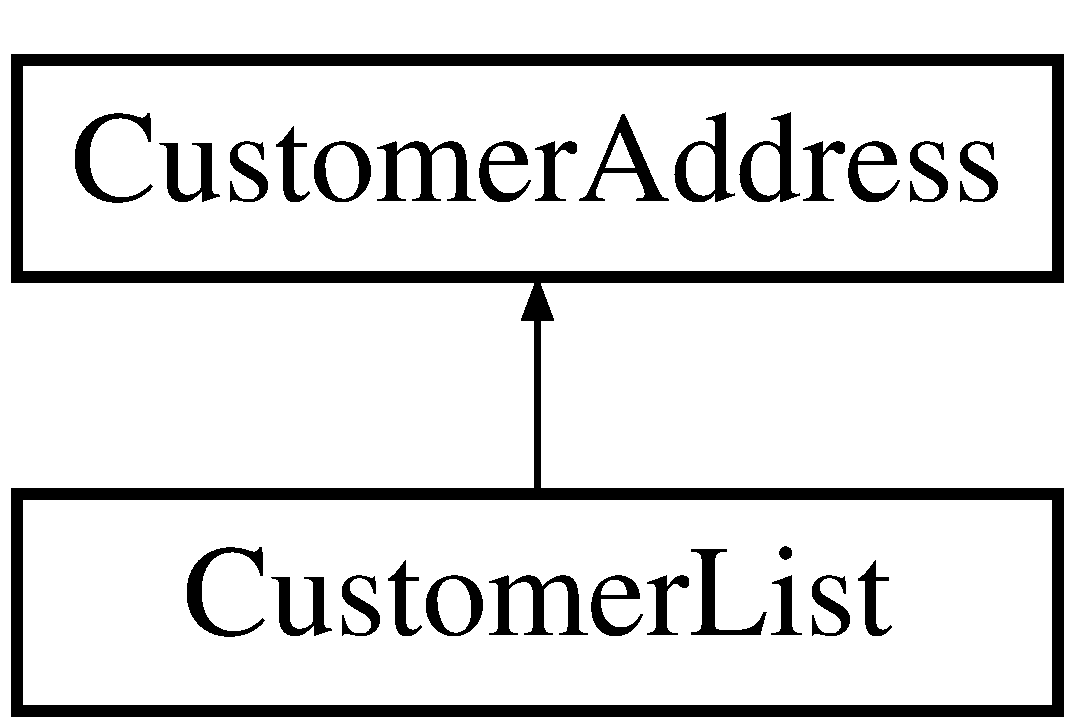
\includegraphics[height=2.000000cm]{class_customer_list}
\end{center}
\end{figure}
\subsection*{Public Member Functions}
\begin{DoxyCompactItemize}
\item 
\mbox{\Hypertarget{class_customer_list_a7d4dd3e97f8f4f0ffe4c4e78e8287961}\label{class_customer_list_a7d4dd3e97f8f4f0ffe4c4e78e8287961}} 
{\bfseries Customer\+List} (Q\+String, Q\+String, Q\+String, Q\+String, int, Q\+String, Q\+String)
\item 
\mbox{\Hypertarget{class_customer_list_a1664cba8e8d632f423af29173d7f129d}\label{class_customer_list_a1664cba8e8d632f423af29173d7f129d}} 
Q\+String {\bfseries Get\+Customer\+Name} () const
\item 
\mbox{\Hypertarget{class_customer_list_ad9c2e6078f443188109172ba3aa194f2}\label{class_customer_list_ad9c2e6078f443188109172ba3aa194f2}} 
Q\+String {\bfseries Get\+Customer\+Interest} () const
\item 
\mbox{\Hypertarget{class_customer_list_a0b5b29392131069645ec640754442134}\label{class_customer_list_a0b5b29392131069645ec640754442134}} 
Q\+String {\bfseries Get\+Customer\+Consider} () const
\end{DoxyCompactItemize}
\subsection*{Private Attributes}
\begin{DoxyCompactItemize}
\item 
\mbox{\Hypertarget{class_customer_list_a2203f4af4c4162680163a4ffa4cae09a}\label{class_customer_list_a2203f4af4c4162680163a4ffa4cae09a}} 
Q\+String {\bfseries customer\+Name}
\item 
\mbox{\Hypertarget{class_customer_list_a7319e26a3596056691229268cc2473a0}\label{class_customer_list_a7319e26a3596056691229268cc2473a0}} 
Q\+String {\bfseries customer\+Interest}
\item 
\mbox{\Hypertarget{class_customer_list_a990624e3c437de3b0771aadffac045ac}\label{class_customer_list_a990624e3c437de3b0771aadffac045ac}} 
Q\+String {\bfseries customer\+Consider}
\end{DoxyCompactItemize}


The documentation for this class was generated from the following files\+:\begin{DoxyCompactItemize}
\item 
C\+:/\+Users/\+Kevin/\+Desktop/project2/customerlist.\+h\item 
C\+:/\+Users/\+Kevin/\+Desktop/project2/customerlist.\+cpp\end{DoxyCompactItemize}

\hypertarget{class_ui_1_1customer_listing}{}\section{Ui\+:\+:customer\+Listing Class Reference}
\label{class_ui_1_1customer_listing}\index{Ui\+::customer\+Listing@{Ui\+::customer\+Listing}}
Inheritance diagram for Ui\+:\+:customer\+Listing\+:\begin{figure}[H]
\begin{center}
\leavevmode
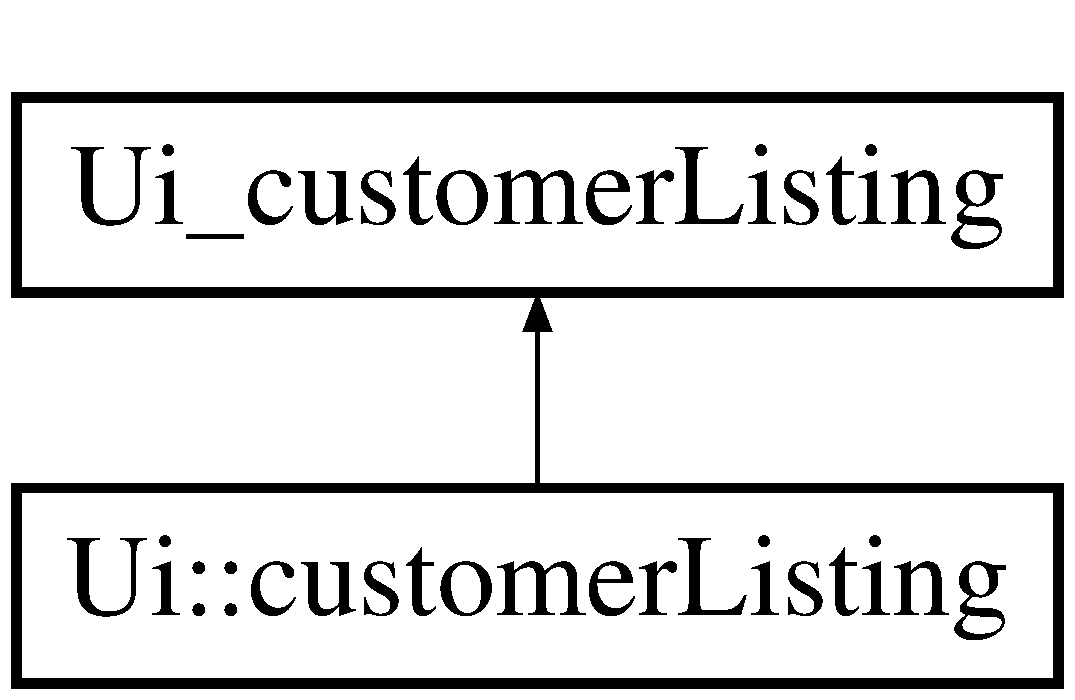
\includegraphics[height=2.000000cm]{class_ui_1_1customer_listing}
\end{center}
\end{figure}
\subsection*{Additional Inherited Members}


The documentation for this class was generated from the following file\+:\begin{DoxyCompactItemize}
\item 
C\+:/\+Users/\+Kevin/\+Desktop/project2/ui\+\_\+customerlisting.\+h\end{DoxyCompactItemize}

\hypertarget{classcustomer_listing}{}\section{customer\+Listing Class Reference}
\label{classcustomer_listing}\index{customer\+Listing@{customer\+Listing}}


Handles operations for the customer listing page.  




{\ttfamily \#include $<$customerlisting.\+h$>$}

Inheritance diagram for customer\+Listing\+:\begin{figure}[H]
\begin{center}
\leavevmode
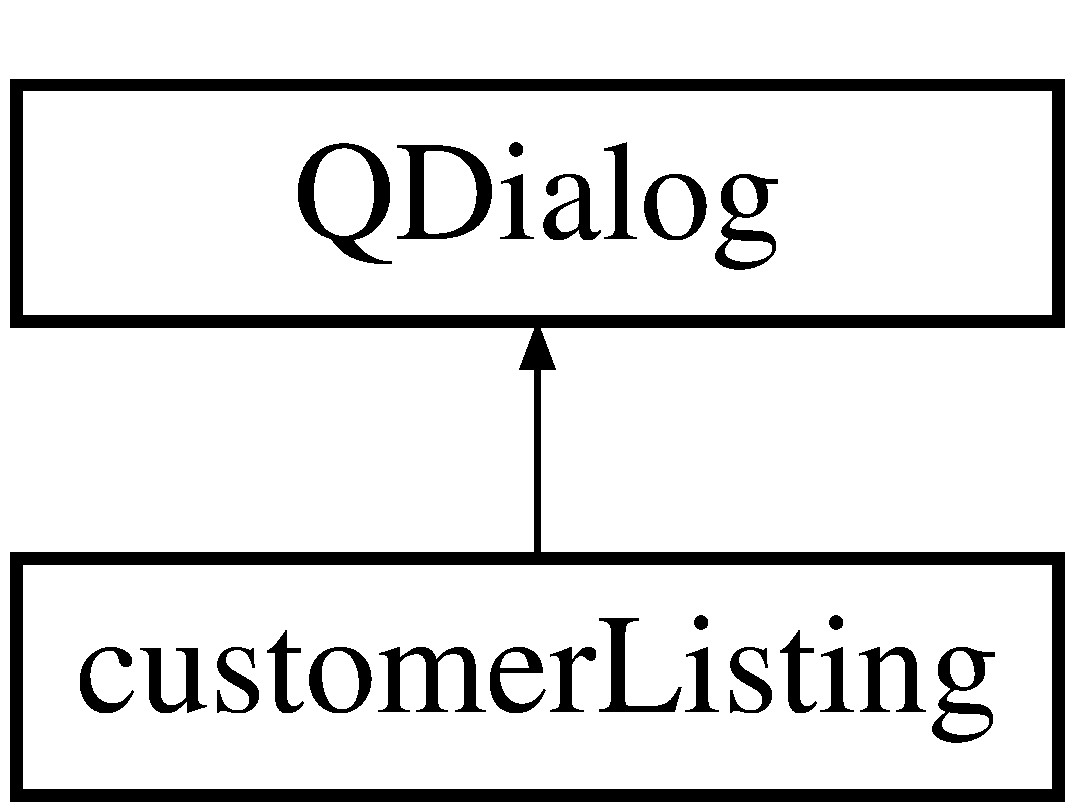
\includegraphics[height=2.000000cm]{classcustomer_listing}
\end{center}
\end{figure}
\subsection*{Public Member Functions}
\begin{DoxyCompactItemize}
\item 
\mbox{\Hypertarget{classcustomer_listing_a0628a9c6898cb9ddd4130ccca331b74a}\label{classcustomer_listing_a0628a9c6898cb9ddd4130ccca331b74a}} 
{\bfseries customer\+Listing} (Q\+Widget $\ast$parent=0)
\end{DoxyCompactItemize}


\subsection{Detailed Description}
Handles operations for the customer listing page. 

The documentation for this class was generated from the following files\+:\begin{DoxyCompactItemize}
\item 
C\+:/\+Users/\+Kevin/\+Documents/\+Git\+Hub/i\+Cyber\+Security/project2/\mbox{\hyperlink{customerlisting_8h}{customerlisting.\+h}}\item 
C\+:/\+Users/\+Kevin/\+Documents/\+Git\+Hub/i\+Cyber\+Security/project2/customerlisting.\+cpp\end{DoxyCompactItemize}

\hypertarget{class_database_manager}{}\section{Database\+Manager Class Reference}
\label{class_database_manager}\index{Database\+Manager@{Database\+Manager}}


Manages data stored within a databse.  




{\ttfamily \#include $<$databasemanager.\+h$>$}

\subsection*{Public Member Functions}
\begin{DoxyCompactItemize}
\item 
\mbox{\Hypertarget{class_database_manager_af1c0598acf843b8e970053f17fc845f1}\label{class_database_manager_af1c0598acf843b8e970053f17fc845f1}} 
bool {\bfseries is\+Open} () const
\item 
\mbox{\Hypertarget{class_database_manager_aefa3d6eae7782904f5d758462b573b1e}\label{class_database_manager_aefa3d6eae7782904f5d758462b573b1e}} 
{\bfseries Database\+Manager} (const \mbox{\hyperlink{class_database_manager}{Database\+Manager}} \&)=delete
\item 
\mbox{\Hypertarget{class_database_manager_acf8defd44bb315a62c6ef9ed10ea52c0}\label{class_database_manager_acf8defd44bb315a62c6ef9ed10ea52c0}} 
void {\bfseries operator=} (const \mbox{\hyperlink{class_database_manager}{Database\+Manager}} \&)=delete
\item 
\mbox{\Hypertarget{class_database_manager_a0355bb13d0608acf18773a6321ed2765}\label{class_database_manager_a0355bb13d0608acf18773a6321ed2765}} 
bool {\bfseries Add\+Customer} (const \mbox{\hyperlink{class_customer_list}{Customer\+List}} \&new\+Customer)
\item 
\mbox{\Hypertarget{class_database_manager_a76c778c9089b97504ea517a575bb95c7}\label{class_database_manager_a76c778c9089b97504ea517a575bb95c7}} 
bool {\bfseries Remove\+Customer} (const \mbox{\hyperlink{class_customer_list}{Customer\+List}} \&customer)
\item 
\mbox{\Hypertarget{class_database_manager_a7e5b964348b1b4b83a20880443a6d714}\label{class_database_manager_a7e5b964348b1b4b83a20880443a6d714}} 
bool {\bfseries customer\+Exist} (const \mbox{\hyperlink{class_customer_list}{Customer\+List}} \&customer)
\item 
\mbox{\Hypertarget{class_database_manager_a5da7ab3f2b017bb9b2482dc8757cf487}\label{class_database_manager_a5da7ab3f2b017bb9b2482dc8757cf487}} 
bool {\bfseries purchase\+Exist} (Q\+String \&purchaser)
\item 
\mbox{\Hypertarget{class_database_manager_a8c125d96cdb57761e391849c0e3de35d}\label{class_database_manager_a8c125d96cdb57761e391849c0e3de35d}} 
bool {\bfseries Add\+Purchase} (Q\+String Company, Q\+String review)
\item 
\mbox{\Hypertarget{class_database_manager_ad25114d420edce2c5e755594b5da6949}\label{class_database_manager_ad25114d420edce2c5e755594b5da6949}} 
bool {\bfseries Add\+Package} (Q\+String name, Q\+String package, double price)
\end{DoxyCompactItemize}
\subsection*{Static Public Member Functions}
\begin{DoxyCompactItemize}
\item 
\mbox{\Hypertarget{class_database_manager_a4abb527066e28f3928ef45af856e134c}\label{class_database_manager_a4abb527066e28f3928ef45af856e134c}} 
static \mbox{\hyperlink{class_database_manager}{Database\+Manager}} \& {\bfseries instance} ()
\end{DoxyCompactItemize}


\subsection{Detailed Description}
Manages data stored within a databse. 

The documentation for this class was generated from the following files\+:\begin{DoxyCompactItemize}
\item 
C\+:/\+Users/\+Kevin/\+Documents/\+Git\+Hub/i\+Cyber\+Security/project2/\mbox{\hyperlink{databasemanager_8h}{databasemanager.\+h}}\item 
C\+:/\+Users/\+Kevin/\+Documents/\+Git\+Hub/i\+Cyber\+Security/project2/databasemanager.\+cpp\end{DoxyCompactItemize}

\hypertarget{class_main_window}{}\section{Main\+Window Class Reference}
\label{class_main_window}\index{Main\+Window@{Main\+Window}}
Inheritance diagram for Main\+Window\+:\begin{figure}[H]
\begin{center}
\leavevmode
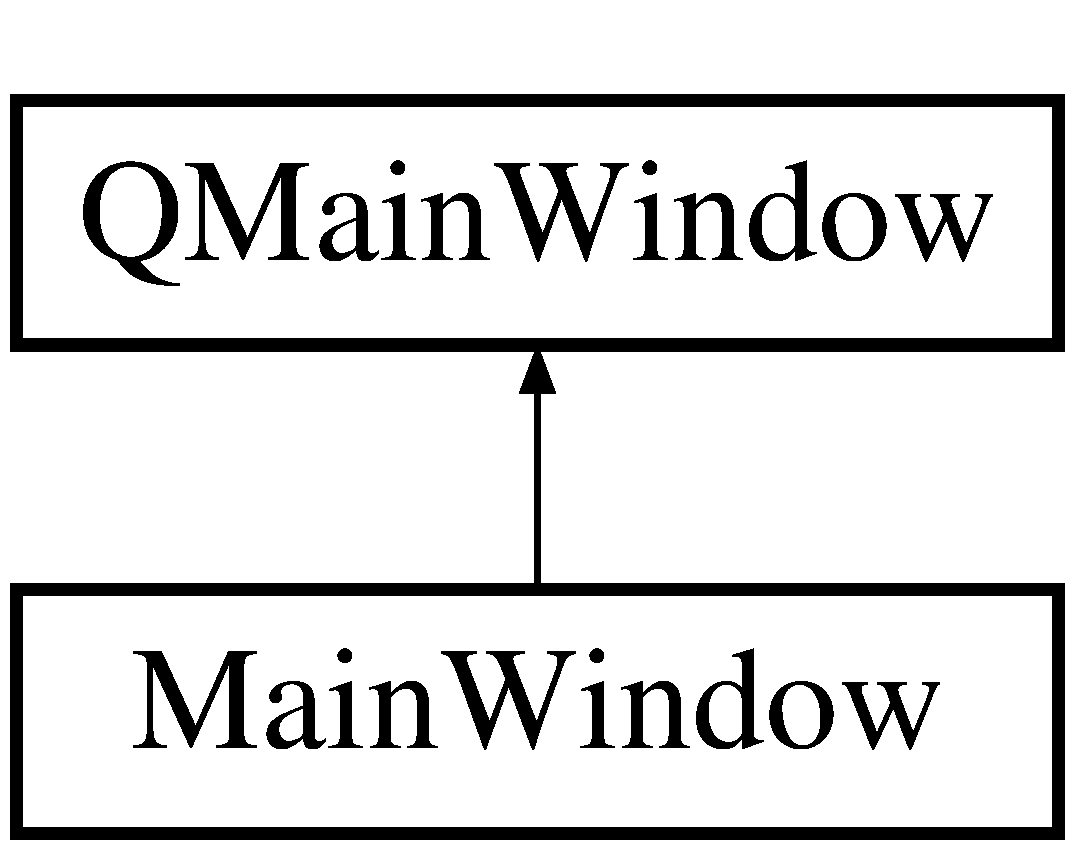
\includegraphics[height=2.000000cm]{class_main_window}
\end{center}
\end{figure}
\subsection*{Public Member Functions}
\begin{DoxyCompactItemize}
\item 
\mbox{\Hypertarget{class_main_window_a8b244be8b7b7db1b08de2a2acb9409db}\label{class_main_window_a8b244be8b7b7db1b08de2a2acb9409db}} 
{\bfseries Main\+Window} (Q\+Widget $\ast$parent=0)
\end{DoxyCompactItemize}
\subsection*{Private Slots}
\begin{DoxyCompactItemize}
\item 
\mbox{\Hypertarget{class_main_window_a6ec8f05cde405e7ba6fcee50da8d0caa}\label{class_main_window_a6ec8f05cde405e7ba6fcee50da8d0caa}} 
void {\bfseries on\+\_\+\+Add\+Item\+\_\+clicked} ()
\item 
\mbox{\Hypertarget{class_main_window_a55b540480cc9dce7e7529a2382281c46}\label{class_main_window_a55b540480cc9dce7e7529a2382281c46}} 
void {\bfseries on\+\_\+\+Delete\+Customer\+\_\+clicked} ()
\item 
\mbox{\Hypertarget{class_main_window_aa464beddd4fe4c4404a1d6fd43f02db7}\label{class_main_window_aa464beddd4fe4c4404a1d6fd43f02db7}} 
void {\bfseries on\+\_\+search\+Customer\+\_\+clicked} ()
\item 
\mbox{\Hypertarget{class_main_window_a0686fc967549d67dfdff36cd8707afc3}\label{class_main_window_a0686fc967549d67dfdff36cd8707afc3}} 
void {\bfseries on\+\_\+load\+Customer\+List\+By\+Name\+\_\+clicked} ()
\item 
\mbox{\Hypertarget{class_main_window_a761479ba0c46f0ef0e391c574527df08}\label{class_main_window_a761479ba0c46f0ef0e391c574527df08}} 
void {\bfseries on\+\_\+load\+Customer\+List\+By\+Key\+\_\+clicked} ()
\item 
\mbox{\Hypertarget{class_main_window_ad329b9928741bf1af1668148b769a7a9}\label{class_main_window_ad329b9928741bf1af1668148b769a7a9}} 
void {\bfseries on\+\_\+admin\+\_\+button\+\_\+clicked} ()
\item 
\mbox{\Hypertarget{class_main_window_aba26165dc8104d3739fa1c48d1f72178}\label{class_main_window_aba26165dc8104d3739fa1c48d1f72178}} 
void {\bfseries on\+\_\+push\+Button\+\_\+login\+\_\+clicked} ()
\item 
\mbox{\Hypertarget{class_main_window_a4d9ea9d5df8ed5e3c3acd7cecc1384e3}\label{class_main_window_a4d9ea9d5df8ed5e3c3acd7cecc1384e3}} 
void {\bfseries on\+\_\+add\+Delete\+Customer\+\_\+\+Button\+\_\+clicked} ()
\item 
\mbox{\Hypertarget{class_main_window_a47fc32380bafe1eec15b68bc5b2827c5}\label{class_main_window_a47fc32380bafe1eec15b68bc5b2827c5}} 
void {\bfseries on\+\_\+add\+Customer\+Back\+Button\+\_\+clicked} ()
\item 
\mbox{\Hypertarget{class_main_window_a5e4260cf98783e4a26bdd954a79aa9d5}\label{class_main_window_a5e4260cf98783e4a26bdd954a79aa9d5}} 
void {\bfseries on\+\_\+search\+Customer\+Back\+Button\+\_\+3\+\_\+clicked} ()
\item 
\mbox{\Hypertarget{class_main_window_a65c4012415c2915c6623cad3b1cec478}\label{class_main_window_a65c4012415c2915c6623cad3b1cec478}} 
void {\bfseries on\+\_\+delete\+Customer\+Back\+Button\+\_\+2\+\_\+clicked} ()
\item 
\mbox{\Hypertarget{class_main_window_a4174976ca43e7aad31bedaedd0639a9b}\label{class_main_window_a4174976ca43e7aad31bedaedd0639a9b}} 
void {\bfseries on\+\_\+list\+By\+Key\+Back\+Button\+\_\+clicked} ()
\item 
\mbox{\Hypertarget{class_main_window_a017555d3eaf72b7ca77522ec661bce93}\label{class_main_window_a017555d3eaf72b7ca77522ec661bce93}} 
void {\bfseries on\+\_\+list\+By\+Name\+Back\+Button\+\_\+clicked} ()
\item 
\mbox{\Hypertarget{class_main_window_ab915ec0529c91b16ba836f8e79172735}\label{class_main_window_ab915ec0529c91b16ba836f8e79172735}} 
void {\bfseries on\+\_\+customer\+List\+\_\+\+Button\+\_\+clicked} ()
\item 
\mbox{\Hypertarget{class_main_window_a13de2ab1da65213246d73b282e6bce47}\label{class_main_window_a13de2ab1da65213246d73b282e6bce47}} 
void {\bfseries on\+\_\+\+Interest\+Combo\+Box\+\_\+activated} (int index)
\item 
\mbox{\Hypertarget{class_main_window_abbe03819dea394cf93ea60c266e058d5}\label{class_main_window_abbe03819dea394cf93ea60c266e058d5}} 
void {\bfseries on\+\_\+consideration\+Combo\+Box\+\_\+activated} (int index)
\item 
\mbox{\Hypertarget{class_main_window_ab5ec4a06e4e38781eb7b913fed92733e}\label{class_main_window_ab5ec4a06e4e38781eb7b913fed92733e}} 
void {\bfseries on\+\_\+tab\+Widget\+\_\+current\+Changed} (int index)
\item 
\mbox{\Hypertarget{class_main_window_a738c75b6db1208e2378a539403c6aff9}\label{class_main_window_a738c75b6db1208e2378a539403c6aff9}} 
void {\bfseries on\+\_\+tab\+Widget\+\_\+tab\+Bar\+Clicked} (int index)
\item 
\mbox{\Hypertarget{class_main_window_a6c6d8a61a24b0d33cb871c9e32b100c5}\label{class_main_window_a6c6d8a61a24b0d33cb871c9e32b100c5}} 
void {\bfseries on\+\_\+\+Load\+All\+Customers\+\_\+clicked} ()
\item 
\mbox{\Hypertarget{class_main_window_a504c5eacab0a182004f2b6832ef70455}\label{class_main_window_a504c5eacab0a182004f2b6832ef70455}} 
void {\bfseries on\+\_\+\+All\+Customers\+Back\+\_\+clicked} ()
\item 
\mbox{\Hypertarget{class_main_window_aaa84473b8e95d3daecf19c98d2d93fdf}\label{class_main_window_aaa84473b8e95d3daecf19c98d2d93fdf}} 
void {\bfseries on\+\_\+search\+Customer\+To\+Update\+\_\+clicked} ()
\item 
\mbox{\Hypertarget{class_main_window_ab6a0ec26c4c5077bf9c3bd604030cb98}\label{class_main_window_ab6a0ec26c4c5077bf9c3bd604030cb98}} 
void {\bfseries on\+\_\+update\+Customer\+\_\+\+Button\+\_\+clicked} ()
\item 
\mbox{\Hypertarget{class_main_window_a278add9518a4d8728056e5658341f694}\label{class_main_window_a278add9518a4d8728056e5658341f694}} 
void {\bfseries on\+\_\+update\+Customer\+Database\+\_\+clicked} ()
\item 
\mbox{\Hypertarget{class_main_window_a8279de9cb0d0a050e3e2e01cc3ff3c22}\label{class_main_window_a8279de9cb0d0a050e3e2e01cc3ff3c22}} 
void {\bfseries on\+\_\+intro\+\_\+clicked} ()
\item 
\mbox{\Hypertarget{class_main_window_a43fac9cd5cabb59c84c2267f5da5e8e3}\label{class_main_window_a43fac9cd5cabb59c84c2267f5da5e8e3}} 
void {\bfseries on\+\_\+purchase\+\_\+clicked} ()
\item 
\mbox{\Hypertarget{class_main_window_ad68ce9e7ba575a4979df4f74bad3efc2}\label{class_main_window_ad68ce9e7ba575a4979df4f74bad3efc2}} 
void {\bfseries on\+\_\+compatability\+\_\+home\+\_\+clicked} ()
\item 
\mbox{\Hypertarget{class_main_window_a65558d7d3f49458f039ed56b863b6f9f}\label{class_main_window_a65558d7d3f49458f039ed56b863b6f9f}} 
void {\bfseries on\+\_\+reviews\+\_\+clicked} ()
\item 
\mbox{\Hypertarget{class_main_window_a68ce9e0c8f9a154d822ad631a4400607}\label{class_main_window_a68ce9e0c8f9a154d822ad631a4400607}} 
void {\bfseries on\+\_\+guarantee\+\_\+clicked} ()
\item 
\mbox{\Hypertarget{class_main_window_afaa483412b8fb7fd0635698cea07b624}\label{class_main_window_afaa483412b8fb7fd0635698cea07b624}} 
void {\bfseries on\+\_\+help\+\_\+clicked} ()
\item 
\mbox{\Hypertarget{class_main_window_acff4fd21883f39eaa0cadd61d4331d2e}\label{class_main_window_acff4fd21883f39eaa0cadd61d4331d2e}} 
void {\bfseries on\+\_\+help\+\_\+exit\+\_\+clicked} ()
\item 
\mbox{\Hypertarget{class_main_window_a95444c9c2e0fde460271c6cb0b8126fa}\label{class_main_window_a95444c9c2e0fde460271c6cb0b8126fa}} 
void {\bfseries on\+\_\+guarantee\+\_\+exit\+\_\+clicked} ()
\item 
\mbox{\Hypertarget{class_main_window_aa636c03838477fad545819908f34d007}\label{class_main_window_aa636c03838477fad545819908f34d007}} 
void {\bfseries on\+\_\+review\+\_\+exit\+\_\+clicked} ()
\item 
\mbox{\Hypertarget{class_main_window_a00bb1b9bcaecfb90604230bb8be0b2f2}\label{class_main_window_a00bb1b9bcaecfb90604230bb8be0b2f2}} 
void {\bfseries on\+\_\+compatability\+\_\+exit\+\_\+clicked} ()
\item 
\mbox{\Hypertarget{class_main_window_a560113571bb9394db779e191a8f9e346}\label{class_main_window_a560113571bb9394db779e191a8f9e346}} 
void {\bfseries on\+\_\+purchase\+\_\+exit\+\_\+clicked} ()
\item 
\mbox{\Hypertarget{class_main_window_a6a67540278c1a486728f06aef2637387}\label{class_main_window_a6a67540278c1a486728f06aef2637387}} 
void {\bfseries on\+\_\+intro\+\_\+exit\+\_\+clicked} ()
\item 
\mbox{\Hypertarget{class_main_window_ad645b24ad5d2c887d4e42306ef9d90b9}\label{class_main_window_ad645b24ad5d2c887d4e42306ef9d90b9}} 
void {\bfseries on\+\_\+update\+Customer\+Back\+Button\+\_\+clicked} ()
\item 
\mbox{\Hypertarget{class_main_window_a319e4c96a5881fc79c623d330ed5d726}\label{class_main_window_a319e4c96a5881fc79c623d330ed5d726}} 
void {\bfseries on\+\_\+admin\+Exit\+\_\+\+Button\+\_\+clicked} ()
\item 
\mbox{\Hypertarget{class_main_window_a48f652d776074ffa13007c1198d515e2}\label{class_main_window_a48f652d776074ffa13007c1198d515e2}} 
void {\bfseries on\+\_\+admin\+Exit\+\_\+clicked} ()
\item 
\mbox{\Hypertarget{class_main_window_a3bc5c9344dfe2a113269663dfce3c0cc}\label{class_main_window_a3bc5c9344dfe2a113269663dfce3c0cc}} 
void {\bfseries on\+\_\+load\+Purchases\+\_\+clicked} ()
\item 
\mbox{\Hypertarget{class_main_window_a2bb3daa29df6f17a15048f35930bdaea}\label{class_main_window_a2bb3daa29df6f17a15048f35930bdaea}} 
void {\bfseries on\+\_\+review\+Back\+Button\+\_\+clicked} ()
\item 
\mbox{\Hypertarget{class_main_window_a50968124cfea882671979c9b9cd603db}\label{class_main_window_a50968124cfea882671979c9b9cd603db}} 
void {\bfseries on\+\_\+leave\+Your\+Review\+\_\+clicked} ()
\item 
\mbox{\Hypertarget{class_main_window_a4de79c63c7fa0b8d7c468ac71f20be81}\label{class_main_window_a4de79c63c7fa0b8d7c468ac71f20be81}} 
void {\bfseries on\+\_\+push\+Button\+\_\+clicked} ()
\item 
\mbox{\Hypertarget{class_main_window_a6ed67aa63c63c4867166cb21115d64f7}\label{class_main_window_a6ed67aa63c63c4867166cb21115d64f7}} 
void {\bfseries on\+\_\+line\+Edit\+\_\+return\+Pressed} ()
\item 
\mbox{\Hypertarget{class_main_window_a105c7ea368b696cb2e166d15f1790394}\label{class_main_window_a105c7ea368b696cb2e166d15f1790394}} 
void {\bfseries on\+\_\+push\+Button\+\_\+purchase\+\_\+clicked} ()
\item 
\mbox{\Hypertarget{class_main_window_a78a121500bf13fe727e3e8e4375c509b}\label{class_main_window_a78a121500bf13fe727e3e8e4375c509b}} 
void {\bfseries on\+\_\+\+Customer\+Tab\+\_\+tab\+Bar\+Clicked} (int index)
\item 
\mbox{\Hypertarget{class_main_window_af4523ace880c4d263f06c7da8b9bc8f6}\label{class_main_window_af4523ace880c4d263f06c7da8b9bc8f6}} 
void {\bfseries on\+\_\+request\+Pamphlet\+\_\+clicked} ()
\item 
\mbox{\Hypertarget{class_main_window_aaf91fab35a1a2e8e6be908bedf8c0af5}\label{class_main_window_aaf91fab35a1a2e8e6be908bedf8c0af5}} 
void {\bfseries on\+\_\+intro\+Tutorial\+\_\+clicked} ()
\item 
\mbox{\Hypertarget{class_main_window_a7ecb35634cefcdbf14f83fdcc1ebf525}\label{class_main_window_a7ecb35634cefcdbf14f83fdcc1ebf525}} 
void {\bfseries on\+\_\+compatability\+Tutorial\+\_\+clicked} ()
\item 
\mbox{\Hypertarget{class_main_window_a24081cae9660b5eb8cddaedeafbc66dd}\label{class_main_window_a24081cae9660b5eb8cddaedeafbc66dd}} 
void {\bfseries on\+\_\+\+Guarantee\+Tutorial\+\_\+clicked} ()
\item 
\mbox{\Hypertarget{class_main_window_af11eef334b3ac8358d1eb8be6cffa60b}\label{class_main_window_af11eef334b3ac8358d1eb8be6cffa60b}} 
void {\bfseries on\+\_\+purchase\+Tutorial\+\_\+clicked} ()
\item 
\mbox{\Hypertarget{class_main_window_aed80016bf2bdaad4dff0205a12f07f10}\label{class_main_window_aed80016bf2bdaad4dff0205a12f07f10}} 
void {\bfseries on\+\_\+review\+Tutorial\+\_\+clicked} ()
\item 
\mbox{\Hypertarget{class_main_window_a96fcd161f1670792c903c9d4a994e279}\label{class_main_window_a96fcd161f1670792c903c9d4a994e279}} 
void {\bfseries on\+\_\+\+Done\+\_\+button\+\_\+clicked} ()
\item 
\mbox{\Hypertarget{class_main_window_a63c4685cc0e0ade70ea78c7a584dd637}\label{class_main_window_a63c4685cc0e0ade70ea78c7a584dd637}} 
void {\bfseries on\+\_\+tutorial\+Push\+Button\+\_\+clicked} ()
\item 
\mbox{\Hypertarget{class_main_window_adf901ae86c89c1e348dfe7fbe9609be8}\label{class_main_window_adf901ae86c89c1e348dfe7fbe9609be8}} 
void {\bfseries on\+\_\+purchase\+Table\+Back\+Button\+\_\+clicked} ()
\item 
\mbox{\Hypertarget{class_main_window_a98d4fd5204351c3fb00762c85419ebaa}\label{class_main_window_a98d4fd5204351c3fb00762c85419ebaa}} 
void {\bfseries on\+\_\+load\+Customers\+By\+Pamplet\+\_\+clicked} ()
\item 
\mbox{\Hypertarget{class_main_window_af56a7b3e24e0ab4019e14bc7c0eeee1b}\label{class_main_window_af56a7b3e24e0ab4019e14bc7c0eeee1b}} 
void {\bfseries on\+\_\+\+Customer\+Pamplet\+Back\+Button\+\_\+clicked} ()
\item 
\mbox{\Hypertarget{class_main_window_ae1bf0b03691b78ed6626e4baf393f9bc}\label{class_main_window_ae1bf0b03691b78ed6626e4baf393f9bc}} 
void {\bfseries on\+\_\+\+Sent\+Pamphlet\+Push\+Button\+\_\+clicked} ()
\item 
\mbox{\Hypertarget{class_main_window_a4b6332f4585f28b5fce0e4738cecc435}\label{class_main_window_a4b6332f4585f28b5fce0e4738cecc435}} 
void {\bfseries on\+\_\+\+Pexit\+\_\+clicked} ()
\end{DoxyCompactItemize}
\subsection*{Private Attributes}
\begin{DoxyCompactItemize}
\item 
\mbox{\Hypertarget{class_main_window_a35466a70ed47252a0191168126a352a5}\label{class_main_window_a35466a70ed47252a0191168126a352a5}} 
\mbox{\hyperlink{class_ui_1_1_main_window}{Ui\+::\+Main\+Window}} $\ast$ {\bfseries ui}
\end{DoxyCompactItemize}


The documentation for this class was generated from the following files\+:\begin{DoxyCompactItemize}
\item 
C\+:/\+Users/\+Kevin/\+Desktop/project2/mainwindow.\+h\item 
C\+:/\+Users/\+Kevin/\+Desktop/project2/mainwindow.\+cpp\end{DoxyCompactItemize}

\hypertarget{class_ui_1_1_main_window}{}\section{Ui\+:\+:Main\+Window Class Reference}
\label{class_ui_1_1_main_window}\index{Ui\+::\+Main\+Window@{Ui\+::\+Main\+Window}}
Inheritance diagram for Ui\+:\+:Main\+Window\+:\begin{figure}[H]
\begin{center}
\leavevmode
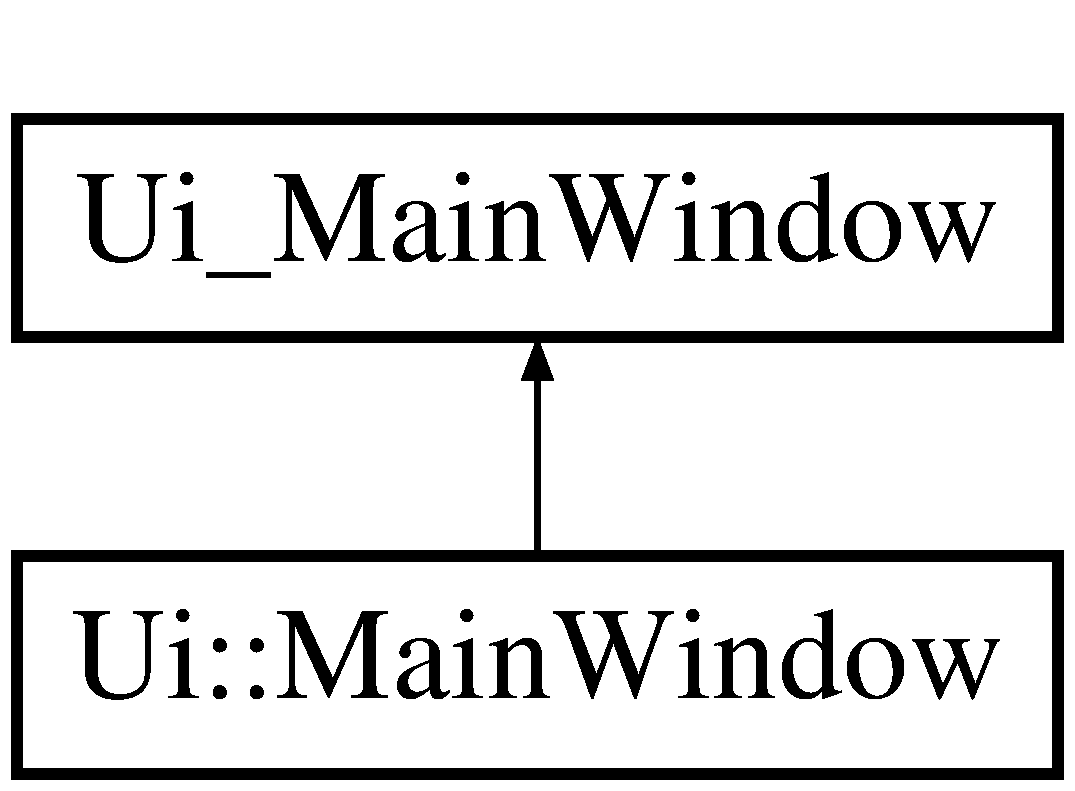
\includegraphics[height=2.000000cm]{class_ui_1_1_main_window}
\end{center}
\end{figure}
\subsection*{Additional Inherited Members}


The documentation for this class was generated from the following file\+:\begin{DoxyCompactItemize}
\item 
C\+:/\+Users/\+Kevin/\+Documents/\+Git\+Hub/i\+Cyber\+Security/project2/ui\+\_\+mainwindow.\+h\end{DoxyCompactItemize}

\hypertarget{class_services}{}\section{Services Class Reference}
\label{class_services}\index{Services@{Services}}


Holds property values for a type of service.  




{\ttfamily \#include $<$services.\+h$>$}

\subsection*{Public Member Functions}
\begin{DoxyCompactItemize}
\item 
\mbox{\Hypertarget{class_services_af3f011adec7bb879dbe2edd7d82c3189}\label{class_services_af3f011adec7bb879dbe2edd7d82c3189}} 
{\bfseries Services} (Q\+String, double)
\end{DoxyCompactItemize}


\subsection{Detailed Description}
Holds property values for a type of service. 

The documentation for this class was generated from the following files\+:\begin{DoxyCompactItemize}
\item 
C\+:/\+Users/\+Kevin/\+Documents/\+Git\+Hub/i\+Cyber\+Security/project2/\mbox{\hyperlink{services_8h}{services.\+h}}\item 
C\+:/\+Users/\+Kevin/\+Documents/\+Git\+Hub/i\+Cyber\+Security/project2/services.\+cpp\end{DoxyCompactItemize}

\hypertarget{class_ui__customer_listing}{}\section{Ui\+\_\+customer\+Listing Class Reference}
\label{class_ui__customer_listing}\index{Ui\+\_\+customer\+Listing@{Ui\+\_\+customer\+Listing}}
Inheritance diagram for Ui\+\_\+customer\+Listing\+:\begin{figure}[H]
\begin{center}
\leavevmode
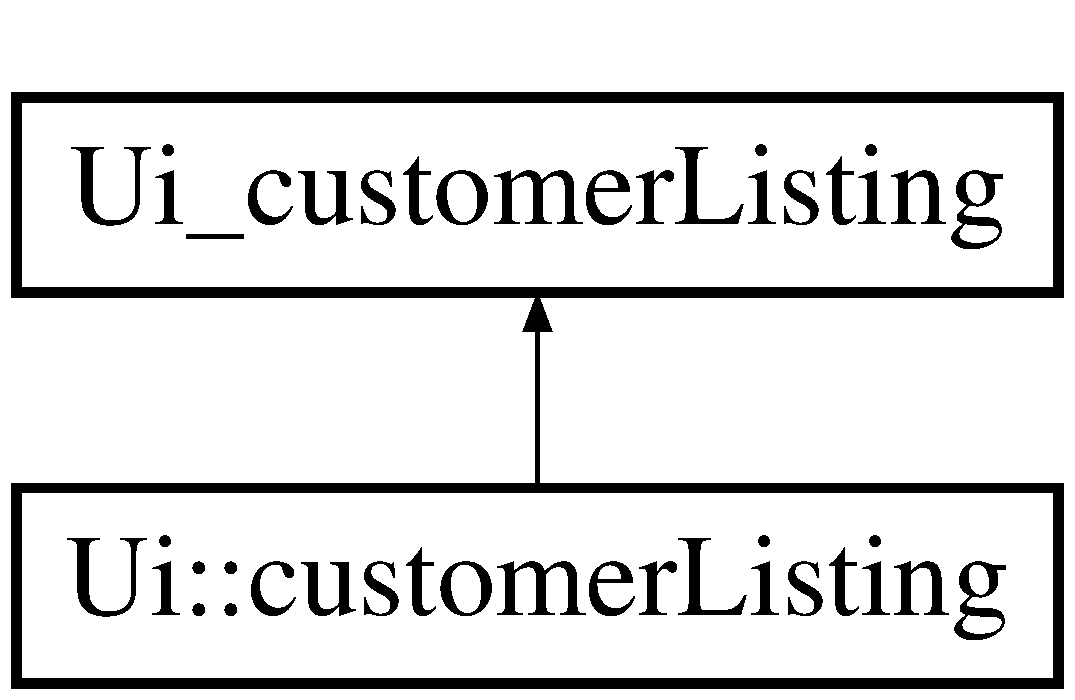
\includegraphics[height=2.000000cm]{class_ui__customer_listing}
\end{center}
\end{figure}
\subsection*{Public Member Functions}
\begin{DoxyCompactItemize}
\item 
\mbox{\Hypertarget{class_ui__customer_listing_acb479d6d68fafdca3c284726d0117add}\label{class_ui__customer_listing_acb479d6d68fafdca3c284726d0117add}} 
void {\bfseries setup\+Ui} (Q\+Dialog $\ast$\mbox{\hyperlink{classcustomer_listing}{customer\+Listing}})
\item 
\mbox{\Hypertarget{class_ui__customer_listing_a617f942f355bf6b0cec7cc9e95d735c9}\label{class_ui__customer_listing_a617f942f355bf6b0cec7cc9e95d735c9}} 
void {\bfseries retranslate\+Ui} (Q\+Dialog $\ast$\mbox{\hyperlink{classcustomer_listing}{customer\+Listing}})
\end{DoxyCompactItemize}
\subsection*{Public Attributes}
\begin{DoxyCompactItemize}
\item 
\mbox{\Hypertarget{class_ui__customer_listing_a3099c0d6cb377cea7162dcb83dc9b367}\label{class_ui__customer_listing_a3099c0d6cb377cea7162dcb83dc9b367}} 
Q\+Table\+Widget $\ast$ {\bfseries customer\+Table2}
\item 
\mbox{\Hypertarget{class_ui__customer_listing_a7f1118df4279405418bc8315b723c5a8}\label{class_ui__customer_listing_a7f1118df4279405418bc8315b723c5a8}} 
Q\+Table\+View $\ast$ {\bfseries customer\+Table}
\item 
\mbox{\Hypertarget{class_ui__customer_listing_a2e0b51ea96979e2703d76a46d0c31d89}\label{class_ui__customer_listing_a2e0b51ea96979e2703d76a46d0c31d89}} 
Q\+Widget $\ast$ {\bfseries widget}
\item 
\mbox{\Hypertarget{class_ui__customer_listing_acbf129d332991405257dddef2ff95b60}\label{class_ui__customer_listing_acbf129d332991405257dddef2ff95b60}} 
Q\+H\+Box\+Layout $\ast$ {\bfseries horizontal\+Layout}
\item 
\mbox{\Hypertarget{class_ui__customer_listing_a4b1909055e76fd455b5ce7036dd9293d}\label{class_ui__customer_listing_a4b1909055e76fd455b5ce7036dd9293d}} 
Q\+Push\+Button $\ast$ {\bfseries View\+All\+Customer}
\item 
\mbox{\Hypertarget{class_ui__customer_listing_a30baffe9fe7b34adceab714d7345a7b6}\label{class_ui__customer_listing_a30baffe9fe7b34adceab714d7345a7b6}} 
Q\+Push\+Button $\ast$ {\bfseries Sortby\+Name}
\item 
\mbox{\Hypertarget{class_ui__customer_listing_aacd8bf39448730821f9a7fc2ba383424}\label{class_ui__customer_listing_aacd8bf39448730821f9a7fc2ba383424}} 
Q\+Push\+Button $\ast$ {\bfseries Sortby\+Key}
\item 
\mbox{\Hypertarget{class_ui__customer_listing_a5a05b551507a3c922e6364f0a89ba87f}\label{class_ui__customer_listing_a5a05b551507a3c922e6364f0a89ba87f}} 
Q\+Push\+Button $\ast$ {\bfseries Sortby\+Pamphlet}
\end{DoxyCompactItemize}


The documentation for this class was generated from the following file\+:\begin{DoxyCompactItemize}
\item 
C\+:/\+Users/\+Kevin/\+Desktop/project2/ui\+\_\+customerlisting.\+h\end{DoxyCompactItemize}

\hypertarget{class_ui___main_window}{}\section{Ui\+\_\+\+Main\+Window Class Reference}
\label{class_ui___main_window}\index{Ui\+\_\+\+Main\+Window@{Ui\+\_\+\+Main\+Window}}
Inheritance diagram for Ui\+\_\+\+Main\+Window\+:\begin{figure}[H]
\begin{center}
\leavevmode
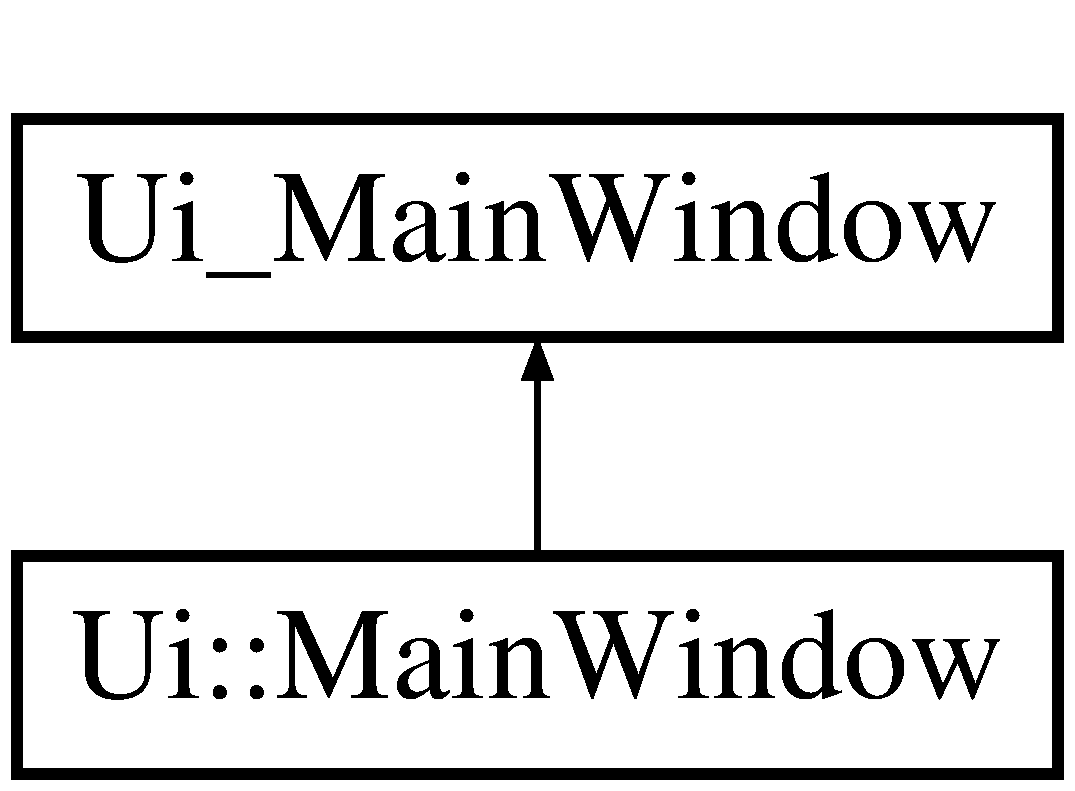
\includegraphics[height=2.000000cm]{class_ui___main_window}
\end{center}
\end{figure}
\subsection*{Public Member Functions}
\begin{DoxyCompactItemize}
\item 
\mbox{\Hypertarget{class_ui___main_window_acf4a0872c4c77d8f43a2ec66ed849b58}\label{class_ui___main_window_acf4a0872c4c77d8f43a2ec66ed849b58}} 
void {\bfseries setup\+Ui} (Q\+Main\+Window $\ast$\mbox{\hyperlink{class_main_window}{Main\+Window}})
\item 
\mbox{\Hypertarget{class_ui___main_window_a097dd160c3534a204904cb374412c618}\label{class_ui___main_window_a097dd160c3534a204904cb374412c618}} 
void {\bfseries retranslate\+Ui} (Q\+Main\+Window $\ast$\mbox{\hyperlink{class_main_window}{Main\+Window}})
\end{DoxyCompactItemize}
\subsection*{Public Attributes}
\begin{DoxyCompactItemize}
\item 
\mbox{\Hypertarget{class_ui___main_window_a30075506c2116c3ed4ff25e07ae75f81}\label{class_ui___main_window_a30075506c2116c3ed4ff25e07ae75f81}} 
Q\+Widget $\ast$ {\bfseries central\+Widget}
\item 
\mbox{\Hypertarget{class_ui___main_window_a8d440a6df1de0bc57afcdda7476d8f19}\label{class_ui___main_window_a8d440a6df1de0bc57afcdda7476d8f19}} 
Q\+Stacked\+Widget $\ast$ {\bfseries stacked\+Widget}
\item 
\mbox{\Hypertarget{class_ui___main_window_a3ec68d4c89c6dcd4fa343bfc486ce351}\label{class_ui___main_window_a3ec68d4c89c6dcd4fa343bfc486ce351}} 
Q\+Widget $\ast$ {\bfseries Home}
\item 
\mbox{\Hypertarget{class_ui___main_window_aef7cb3be8cecfc9aaf98f036a98781ce}\label{class_ui___main_window_aef7cb3be8cecfc9aaf98f036a98781ce}} 
Q\+Group\+Box $\ast$ {\bfseries group\+Box}
\item 
\mbox{\Hypertarget{class_ui___main_window_a29d4f23d897d76f4722e7702cf290e96}\label{class_ui___main_window_a29d4f23d897d76f4722e7702cf290e96}} 
Q\+Push\+Button $\ast$ {\bfseries admin\+\_\+button}
\item 
\mbox{\Hypertarget{class_ui___main_window_aee9f42af99553b2f02ca79b5743785b4}\label{class_ui___main_window_aee9f42af99553b2f02ca79b5743785b4}} 
Q\+Push\+Button $\ast$ {\bfseries intro}
\item 
\mbox{\Hypertarget{class_ui___main_window_ac2a962d000aca877f10f86d0280d6918}\label{class_ui___main_window_ac2a962d000aca877f10f86d0280d6918}} 
Q\+Push\+Button $\ast$ {\bfseries compatability\+\_\+home}
\item 
\mbox{\Hypertarget{class_ui___main_window_a9b06eeec5a6f87bcd5734ef0e54866d5}\label{class_ui___main_window_a9b06eeec5a6f87bcd5734ef0e54866d5}} 
Q\+Push\+Button $\ast$ {\bfseries reviews}
\item 
\mbox{\Hypertarget{class_ui___main_window_ac7278e03d5f64c64ceff38f64edfced1}\label{class_ui___main_window_ac7278e03d5f64c64ceff38f64edfced1}} 
Q\+Push\+Button $\ast$ {\bfseries help}
\item 
\mbox{\Hypertarget{class_ui___main_window_a85fdf25efb0f619da072b603d1dbe9e8}\label{class_ui___main_window_a85fdf25efb0f619da072b603d1dbe9e8}} 
Q\+Push\+Button $\ast$ {\bfseries guarantee}
\item 
\mbox{\Hypertarget{class_ui___main_window_a34d28f0ee046a4395f033d5f9f5fa111}\label{class_ui___main_window_a34d28f0ee046a4395f033d5f9f5fa111}} 
Q\+Push\+Button $\ast$ {\bfseries purchase}
\item 
\mbox{\Hypertarget{class_ui___main_window_a67bf89304057cc9a572af380f4c2e81e}\label{class_ui___main_window_a67bf89304057cc9a572af380f4c2e81e}} 
Q\+Push\+Button $\ast$ {\bfseries request\+Pamphlet}
\item 
\mbox{\Hypertarget{class_ui___main_window_a9a97c6d9a8bced056e8664c25f393310}\label{class_ui___main_window_a9a97c6d9a8bced056e8664c25f393310}} 
Q\+Widget $\ast$ {\bfseries Admin\+Login}
\item 
\mbox{\Hypertarget{class_ui___main_window_ad8a919e5634add9c41bfc319cb9fd338}\label{class_ui___main_window_ad8a919e5634add9c41bfc319cb9fd338}} 
Q\+Group\+Box $\ast$ {\bfseries group\+Box\+\_\+4}
\item 
\mbox{\Hypertarget{class_ui___main_window_a0e90c7e9ad77386881e0b264ddb9dd22}\label{class_ui___main_window_a0e90c7e9ad77386881e0b264ddb9dd22}} 
Q\+Label $\ast$ {\bfseries label\+\_\+9}
\item 
\mbox{\Hypertarget{class_ui___main_window_ada6a6ee374998f8c4edc4c5750b690e9}\label{class_ui___main_window_ada6a6ee374998f8c4edc4c5750b690e9}} 
Q\+Line\+Edit $\ast$ {\bfseries line\+Edit\+\_\+username}
\item 
\mbox{\Hypertarget{class_ui___main_window_ab0fe5a3bb0fbeb730223449fcd69ed27}\label{class_ui___main_window_ab0fe5a3bb0fbeb730223449fcd69ed27}} 
Q\+Line\+Edit $\ast$ {\bfseries line\+Edit\+\_\+password}
\item 
\mbox{\Hypertarget{class_ui___main_window_a9dc4dba26b83e0c94aa566e1c564420b}\label{class_ui___main_window_a9dc4dba26b83e0c94aa566e1c564420b}} 
Q\+Label $\ast$ {\bfseries label\+\_\+10}
\item 
\mbox{\Hypertarget{class_ui___main_window_a4f12a71b4a2fb6f85df2300d83b5ed3e}\label{class_ui___main_window_a4f12a71b4a2fb6f85df2300d83b5ed3e}} 
Q\+Label $\ast$ {\bfseries label\+\_\+11}
\item 
\mbox{\Hypertarget{class_ui___main_window_ad28b2dacd95cdc7176cc0c702bd26140}\label{class_ui___main_window_ad28b2dacd95cdc7176cc0c702bd26140}} 
Q\+Push\+Button $\ast$ {\bfseries push\+Button\+\_\+login}
\item 
\mbox{\Hypertarget{class_ui___main_window_a4306e546d71f0c2612c22bd0bb5af7cd}\label{class_ui___main_window_a4306e546d71f0c2612c22bd0bb5af7cd}} 
Q\+Label $\ast$ {\bfseries label\+\_\+error}
\item 
\mbox{\Hypertarget{class_ui___main_window_a14547b06f96c9603a83f42f899ee5ab2}\label{class_ui___main_window_a14547b06f96c9603a83f42f899ee5ab2}} 
Q\+Push\+Button $\ast$ {\bfseries admin\+Exit}
\item 
\mbox{\Hypertarget{class_ui___main_window_a9a135a40d5499e76a063f20a0f79376d}\label{class_ui___main_window_a9a135a40d5499e76a063f20a0f79376d}} 
Q\+Widget $\ast$ {\bfseries Admin\+Base}
\item 
\mbox{\Hypertarget{class_ui___main_window_abb28acde35ffce4d0e6152579df2cbc3}\label{class_ui___main_window_abb28acde35ffce4d0e6152579df2cbc3}} 
Q\+Group\+Box $\ast$ {\bfseries group\+Box\+\_\+2}
\item 
\mbox{\Hypertarget{class_ui___main_window_a39c1cd485c97583173618ab1785f6366}\label{class_ui___main_window_a39c1cd485c97583173618ab1785f6366}} 
Q\+Push\+Button $\ast$ {\bfseries admin\+Exit\+\_\+\+Button}
\item 
\mbox{\Hypertarget{class_ui___main_window_a5840c8779252d33e0f56ed1fbf6bae98}\label{class_ui___main_window_a5840c8779252d33e0f56ed1fbf6bae98}} 
Q\+Push\+Button $\ast$ {\bfseries update\+Customer\+\_\+\+Button}
\item 
\mbox{\Hypertarget{class_ui___main_window_ad775a565f6e6be2d30285b35377fecd6}\label{class_ui___main_window_ad775a565f6e6be2d30285b35377fecd6}} 
Q\+Push\+Button $\ast$ {\bfseries add\+Delete\+Customer\+\_\+\+Button}
\item 
\mbox{\Hypertarget{class_ui___main_window_a27d575bd6c10f774c80da3b3982105f3}\label{class_ui___main_window_a27d575bd6c10f774c80da3b3982105f3}} 
Q\+Push\+Button $\ast$ {\bfseries customer\+List\+\_\+\+Button}
\item 
\mbox{\Hypertarget{class_ui___main_window_a89a61d699575279e0ffd7f9b2356acb6}\label{class_ui___main_window_a89a61d699575279e0ffd7f9b2356acb6}} 
Q\+Widget $\ast$ {\bfseries Customer\+Fx}
\item 
\mbox{\Hypertarget{class_ui___main_window_a780faab522f8a2aebde09f541bd39c92}\label{class_ui___main_window_a780faab522f8a2aebde09f541bd39c92}} 
Q\+Label $\ast$ {\bfseries db\+Connect}
\item 
\mbox{\Hypertarget{class_ui___main_window_a6f38f4ef9943a611f7c998ee45db1b83}\label{class_ui___main_window_a6f38f4ef9943a611f7c998ee45db1b83}} 
Q\+Tab\+Widget $\ast$ {\bfseries Add\+Customer}
\item 
\mbox{\Hypertarget{class_ui___main_window_a3efc28c664e9f5115095aafbbc5ac6bc}\label{class_ui___main_window_a3efc28c664e9f5115095aafbbc5ac6bc}} 
Q\+Widget $\ast$ {\bfseries tab}
\item 
\mbox{\Hypertarget{class_ui___main_window_ad9c89133780f28e6efa2ec17ceb9cff5}\label{class_ui___main_window_ad9c89133780f28e6efa2ec17ceb9cff5}} 
Q\+Label $\ast$ {\bfseries label}
\item 
\mbox{\Hypertarget{class_ui___main_window_a2e2516d755e4dd53fc905dabddf2738a}\label{class_ui___main_window_a2e2516d755e4dd53fc905dabddf2738a}} 
Q\+Label $\ast$ {\bfseries label\+\_\+2}
\item 
\mbox{\Hypertarget{class_ui___main_window_a0376fd90247280e7c7957cc70628708c}\label{class_ui___main_window_a0376fd90247280e7c7957cc70628708c}} 
Q\+Label $\ast$ {\bfseries label\+\_\+3}
\item 
\mbox{\Hypertarget{class_ui___main_window_a78c7e10730b43c6700cd7216911ed76a}\label{class_ui___main_window_a78c7e10730b43c6700cd7216911ed76a}} 
Q\+Label $\ast$ {\bfseries label\+\_\+4}
\item 
\mbox{\Hypertarget{class_ui___main_window_ad6bab8fb8903b8f41afea1218ee52695}\label{class_ui___main_window_ad6bab8fb8903b8f41afea1218ee52695}} 
Q\+Label $\ast$ {\bfseries label\+\_\+5}
\item 
\mbox{\Hypertarget{class_ui___main_window_a663f728e6244926a795c6e6892673b1d}\label{class_ui___main_window_a663f728e6244926a795c6e6892673b1d}} 
Q\+Label $\ast$ {\bfseries label\+\_\+6}
\item 
\mbox{\Hypertarget{class_ui___main_window_a13936e6f18b1c90402b3c7a3c92b6cdb}\label{class_ui___main_window_a13936e6f18b1c90402b3c7a3c92b6cdb}} 
Q\+Label $\ast$ {\bfseries label\+\_\+7}
\item 
\mbox{\Hypertarget{class_ui___main_window_a04efde2b4f8cac79a380cba2c283e541}\label{class_ui___main_window_a04efde2b4f8cac79a380cba2c283e541}} 
Q\+Push\+Button $\ast$ {\bfseries Add\+Item}
\item 
\mbox{\Hypertarget{class_ui___main_window_a7ab36d2e9d2017b4b5664383a1a75104}\label{class_ui___main_window_a7ab36d2e9d2017b4b5664383a1a75104}} 
Q\+Label $\ast$ {\bfseries message}
\item 
\mbox{\Hypertarget{class_ui___main_window_a88eb019735d0c675c82d92a7fe20db74}\label{class_ui___main_window_a88eb019735d0c675c82d92a7fe20db74}} 
Q\+Push\+Button $\ast$ {\bfseries add\+Customer\+Back\+Button}
\item 
\mbox{\Hypertarget{class_ui___main_window_ab96ab0f0578098521fa69a75aa5cdde8}\label{class_ui___main_window_ab96ab0f0578098521fa69a75aa5cdde8}} 
Q\+Widget $\ast$ {\bfseries layout\+Widget}
\item 
\mbox{\Hypertarget{class_ui___main_window_a6f40fc110b15410c00837a446d57bdbe}\label{class_ui___main_window_a6f40fc110b15410c00837a446d57bdbe}} 
Q\+V\+Box\+Layout $\ast$ {\bfseries vertical\+Layout\+\_\+4}
\item 
\mbox{\Hypertarget{class_ui___main_window_a47f06bbf333c53711ae19082ead81e57}\label{class_ui___main_window_a47f06bbf333c53711ae19082ead81e57}} 
Q\+Line\+Edit $\ast$ {\bfseries c\+Name}
\item 
\mbox{\Hypertarget{class_ui___main_window_a7e1c5d56e742785f9be25030c0576c74}\label{class_ui___main_window_a7e1c5d56e742785f9be25030c0576c74}} 
Q\+Line\+Edit $\ast$ {\bfseries c\+Street}
\item 
\mbox{\Hypertarget{class_ui___main_window_ac252ddd320023069ce6c95fc9f96917d}\label{class_ui___main_window_ac252ddd320023069ce6c95fc9f96917d}} 
Q\+Line\+Edit $\ast$ {\bfseries c\+City}
\item 
\mbox{\Hypertarget{class_ui___main_window_a07bc1eb21b58683a9aaec0c39688dda6}\label{class_ui___main_window_a07bc1eb21b58683a9aaec0c39688dda6}} 
Q\+Line\+Edit $\ast$ {\bfseries c\+State}
\item 
\mbox{\Hypertarget{class_ui___main_window_a59bb35c1207ffa1e04e04ed76a49b676}\label{class_ui___main_window_a59bb35c1207ffa1e04e04ed76a49b676}} 
Q\+Spin\+Box $\ast$ {\bfseries c\+Zip\+Code}
\item 
\mbox{\Hypertarget{class_ui___main_window_a25248d3ec91aa4dd92dfb92ee8ccaf32}\label{class_ui___main_window_a25248d3ec91aa4dd92dfb92ee8ccaf32}} 
Q\+Combo\+Box $\ast$ {\bfseries Interest\+Combo\+Box}
\item 
\mbox{\Hypertarget{class_ui___main_window_ad19f5985b234e4129634aee2966972b6}\label{class_ui___main_window_ad19f5985b234e4129634aee2966972b6}} 
Q\+Combo\+Box $\ast$ {\bfseries consideration\+Combo\+Box}
\item 
\mbox{\Hypertarget{class_ui___main_window_a1182872adcdb1424c893a8f201eabee4}\label{class_ui___main_window_a1182872adcdb1424c893a8f201eabee4}} 
Q\+Label $\ast$ {\bfseries Add\+Member\+Message}
\item 
\mbox{\Hypertarget{class_ui___main_window_a83495b23cbc6810f81978dc0d584b810}\label{class_ui___main_window_a83495b23cbc6810f81978dc0d584b810}} 
Q\+Widget $\ast$ {\bfseries tab\+\_\+2}
\item 
\mbox{\Hypertarget{class_ui___main_window_a805d415fff07a22a85219e1f22f2da28}\label{class_ui___main_window_a805d415fff07a22a85219e1f22f2da28}} 
Q\+Widget $\ast$ {\bfseries vertical\+Layout\+Widget}
\item 
\mbox{\Hypertarget{class_ui___main_window_aecd96a04789fcfec3f98d80390ad8184}\label{class_ui___main_window_aecd96a04789fcfec3f98d80390ad8184}} 
Q\+V\+Box\+Layout $\ast$ {\bfseries vertical\+Layout}
\item 
\mbox{\Hypertarget{class_ui___main_window_af183bfbfb9f38bbdd60caf92b15e23dc}\label{class_ui___main_window_af183bfbfb9f38bbdd60caf92b15e23dc}} 
Q\+Label $\ast$ {\bfseries label\+\_\+8}
\item 
\mbox{\Hypertarget{class_ui___main_window_a0609806ecf470a0a506cff100a293f5c}\label{class_ui___main_window_a0609806ecf470a0a506cff100a293f5c}} 
Q\+Line\+Edit $\ast$ {\bfseries Delete\+Customer\+Name}
\item 
\mbox{\Hypertarget{class_ui___main_window_a5a892ebccf08983b3f64ebcf82b3c4ff}\label{class_ui___main_window_a5a892ebccf08983b3f64ebcf82b3c4ff}} 
Q\+Push\+Button $\ast$ {\bfseries Delete\+Customer}
\item 
\mbox{\Hypertarget{class_ui___main_window_a50f57d40b6bc88b1f62d774daafa5ed0}\label{class_ui___main_window_a50f57d40b6bc88b1f62d774daafa5ed0}} 
Q\+Label $\ast$ {\bfseries delete\+Message}
\item 
\mbox{\Hypertarget{class_ui___main_window_a1bd01d0820b1695e67cf8a4ac5b920f9}\label{class_ui___main_window_a1bd01d0820b1695e67cf8a4ac5b920f9}} 
Q\+Push\+Button $\ast$ {\bfseries delete\+Customer\+Back\+Button\+\_\+2}
\item 
\mbox{\Hypertarget{class_ui___main_window_a41c7e77dd12b9445e13dbe8fb5ae1488}\label{class_ui___main_window_a41c7e77dd12b9445e13dbe8fb5ae1488}} 
Q\+Widget $\ast$ {\bfseries tab\+\_\+3}
\item 
\mbox{\Hypertarget{class_ui___main_window_a62b94f49d79e473da0f96d804b9c3af7}\label{class_ui___main_window_a62b94f49d79e473da0f96d804b9c3af7}} 
Q\+Widget $\ast$ {\bfseries vertical\+Layout\+Widget\+\_\+2}
\item 
\mbox{\Hypertarget{class_ui___main_window_a0c01bad60d9f422a1258e710635a2f65}\label{class_ui___main_window_a0c01bad60d9f422a1258e710635a2f65}} 
Q\+V\+Box\+Layout $\ast$ {\bfseries vertical\+Layout\+\_\+2}
\item 
\mbox{\Hypertarget{class_ui___main_window_a4124a22ab8d4312bfd587b22c902dbee}\label{class_ui___main_window_a4124a22ab8d4312bfd587b22c902dbee}} 
Q\+Label $\ast$ {\bfseries update\+Customer\+Label}
\item 
\mbox{\Hypertarget{class_ui___main_window_a1339ece316972ffb68d7419fa8540094}\label{class_ui___main_window_a1339ece316972ffb68d7419fa8540094}} 
Q\+Line\+Edit $\ast$ {\bfseries update\+Customer}
\item 
\mbox{\Hypertarget{class_ui___main_window_a10e060af9582abab227c07cc53ff5649}\label{class_ui___main_window_a10e060af9582abab227c07cc53ff5649}} 
Q\+Push\+Button $\ast$ {\bfseries search\+Customer}
\item 
\mbox{\Hypertarget{class_ui___main_window_ae17975d299ee8e068f31c925d265a811}\label{class_ui___main_window_ae17975d299ee8e068f31c925d265a811}} 
Q\+Label $\ast$ {\bfseries search\+Message}
\item 
\mbox{\Hypertarget{class_ui___main_window_af71d593674c287382624ed98ca572c63}\label{class_ui___main_window_af71d593674c287382624ed98ca572c63}} 
Q\+Push\+Button $\ast$ {\bfseries search\+Customer\+Back\+Button\+\_\+3}
\item 
\mbox{\Hypertarget{class_ui___main_window_a1d388e30db212be00e0063731ee64c2b}\label{class_ui___main_window_a1d388e30db212be00e0063731ee64c2b}} 
Q\+Table\+View $\ast$ {\bfseries found\+Customer}
\item 
\mbox{\Hypertarget{class_ui___main_window_afa711e310621dd27692b6747ccfb72a0}\label{class_ui___main_window_afa711e310621dd27692b6747ccfb72a0}} 
Q\+Widget $\ast$ {\bfseries Update\+Customer}
\item 
\mbox{\Hypertarget{class_ui___main_window_a320d3d7ba1cb8fff7b7b95923ed10f5e}\label{class_ui___main_window_a320d3d7ba1cb8fff7b7b95923ed10f5e}} 
Q\+Group\+Box $\ast$ {\bfseries group\+Box\+\_\+3}
\item 
\mbox{\Hypertarget{class_ui___main_window_a1edd82e49c1b4b0153606ef630ececf0}\label{class_ui___main_window_a1edd82e49c1b4b0153606ef630ececf0}} 
Q\+Push\+Button $\ast$ {\bfseries search\+Customer\+To\+Update}
\item 
\mbox{\Hypertarget{class_ui___main_window_acfaf6d66c957965550714c6b9bd0edc0}\label{class_ui___main_window_acfaf6d66c957965550714c6b9bd0edc0}} 
Q\+Widget $\ast$ {\bfseries vertical\+Layout\+Widget\+\_\+3}
\item 
\mbox{\Hypertarget{class_ui___main_window_a38b8a4b887f3b58e2a49e7905ae6f1f0}\label{class_ui___main_window_a38b8a4b887f3b58e2a49e7905ae6f1f0}} 
Q\+V\+Box\+Layout $\ast$ {\bfseries vertical\+Layout\+\_\+3}
\item 
\mbox{\Hypertarget{class_ui___main_window_a82f0ffd8f1bead4614d8511e89b0b9d5}\label{class_ui___main_window_a82f0ffd8f1bead4614d8511e89b0b9d5}} 
Q\+Label $\ast$ {\bfseries update\+Customer\+Label\+\_\+2}
\item 
\mbox{\Hypertarget{class_ui___main_window_a85eab231ee087659c54c83fdb8002055}\label{class_ui___main_window_a85eab231ee087659c54c83fdb8002055}} 
Q\+Line\+Edit $\ast$ {\bfseries update\+Customer\+\_\+2}
\item 
\mbox{\Hypertarget{class_ui___main_window_a42a5f0790625f5505c796972bbe2ac4f}\label{class_ui___main_window_a42a5f0790625f5505c796972bbe2ac4f}} 
Q\+Label $\ast$ {\bfseries update\+Customer\+Found}
\item 
\mbox{\Hypertarget{class_ui___main_window_af56f7d6315c310cc2372580891081c65}\label{class_ui___main_window_af56f7d6315c310cc2372580891081c65}} 
Q\+Push\+Button $\ast$ {\bfseries update\+Customer\+Database}
\item 
\mbox{\Hypertarget{class_ui___main_window_af43f57c2888c29e05110b4c546883602}\label{class_ui___main_window_af43f57c2888c29e05110b4c546883602}} 
Q\+Push\+Button $\ast$ {\bfseries update\+Customer\+Back\+Button}
\item 
\mbox{\Hypertarget{class_ui___main_window_aab31b3dec8d767525dea6f163e029e48}\label{class_ui___main_window_aab31b3dec8d767525dea6f163e029e48}} 
Q\+Widget $\ast$ {\bfseries layout\+Widget1}
\item 
\mbox{\Hypertarget{class_ui___main_window_a525ed3c5fe0784ac502ee222fba4e205}\label{class_ui___main_window_a525ed3c5fe0784ac502ee222fba4e205}} 
Q\+Grid\+Layout $\ast$ {\bfseries grid\+Layout}
\item 
\mbox{\Hypertarget{class_ui___main_window_a93c190b085c63a667c535ba0bbcfec7c}\label{class_ui___main_window_a93c190b085c63a667c535ba0bbcfec7c}} 
Q\+V\+Box\+Layout $\ast$ {\bfseries vertical\+Layout\+\_\+6}
\item 
\mbox{\Hypertarget{class_ui___main_window_a1f4ff90c122fededcc08604401442034}\label{class_ui___main_window_a1f4ff90c122fededcc08604401442034}} 
Q\+Label $\ast$ {\bfseries label\+\_\+17}
\item 
\mbox{\Hypertarget{class_ui___main_window_aa2621565827195e88436fb54220bb48d}\label{class_ui___main_window_aa2621565827195e88436fb54220bb48d}} 
Q\+Label $\ast$ {\bfseries label\+\_\+12}
\item 
\mbox{\Hypertarget{class_ui___main_window_a1c16c0a684617927472e534822a63c7d}\label{class_ui___main_window_a1c16c0a684617927472e534822a63c7d}} 
Q\+Label $\ast$ {\bfseries label\+\_\+14}
\item 
\mbox{\Hypertarget{class_ui___main_window_ab6ac4329a89041f557332f6569d94493}\label{class_ui___main_window_ab6ac4329a89041f557332f6569d94493}} 
Q\+Label $\ast$ {\bfseries label\+\_\+16}
\item 
\mbox{\Hypertarget{class_ui___main_window_a55100f53189f25cf8a1ee0beb29be642}\label{class_ui___main_window_a55100f53189f25cf8a1ee0beb29be642}} 
Q\+Label $\ast$ {\bfseries label\+\_\+18}
\item 
\mbox{\Hypertarget{class_ui___main_window_ac1cbc41e9dbaeb3d0bdc2189d8e9ee1d}\label{class_ui___main_window_ac1cbc41e9dbaeb3d0bdc2189d8e9ee1d}} 
Q\+Label $\ast$ {\bfseries label\+\_\+13}
\item 
\mbox{\Hypertarget{class_ui___main_window_a882200d8ae16962f5dd3b749ebacbf7e}\label{class_ui___main_window_a882200d8ae16962f5dd3b749ebacbf7e}} 
Q\+Label $\ast$ {\bfseries label\+\_\+15}
\item 
\mbox{\Hypertarget{class_ui___main_window_afcc20a3d5058037a00cdc6122f231848}\label{class_ui___main_window_afcc20a3d5058037a00cdc6122f231848}} 
Q\+V\+Box\+Layout $\ast$ {\bfseries vertical\+Layout\+\_\+5}
\item 
\mbox{\Hypertarget{class_ui___main_window_a9a70e56f3f3a41b45871579bf0183f14}\label{class_ui___main_window_a9a70e56f3f3a41b45871579bf0183f14}} 
Q\+Line\+Edit $\ast$ {\bfseries c\+Name\+\_\+2}
\item 
\mbox{\Hypertarget{class_ui___main_window_a7b67a1664ba294396c851565bb1c247c}\label{class_ui___main_window_a7b67a1664ba294396c851565bb1c247c}} 
Q\+Line\+Edit $\ast$ {\bfseries c\+Street\+\_\+2}
\item 
\mbox{\Hypertarget{class_ui___main_window_a97860074e1ee4617de65ffca839e30e4}\label{class_ui___main_window_a97860074e1ee4617de65ffca839e30e4}} 
Q\+Line\+Edit $\ast$ {\bfseries c\+City\+\_\+2}
\item 
\mbox{\Hypertarget{class_ui___main_window_ac2ee24b214782f40912f859f1e87b4f6}\label{class_ui___main_window_ac2ee24b214782f40912f859f1e87b4f6}} 
Q\+Line\+Edit $\ast$ {\bfseries c\+State\+\_\+2}
\item 
\mbox{\Hypertarget{class_ui___main_window_a987987023a94b8ae38924f08bc3f4b03}\label{class_ui___main_window_a987987023a94b8ae38924f08bc3f4b03}} 
Q\+Spin\+Box $\ast$ {\bfseries c\+Zip\+Code\+\_\+2}
\item 
\mbox{\Hypertarget{class_ui___main_window_a673af35ada1b4e455533baa327ff7aed}\label{class_ui___main_window_a673af35ada1b4e455533baa327ff7aed}} 
Q\+Combo\+Box $\ast$ {\bfseries Interest\+Combo\+Box\+\_\+2}
\item 
\mbox{\Hypertarget{class_ui___main_window_a27d5334a330bd73370eea70beed090a5}\label{class_ui___main_window_a27d5334a330bd73370eea70beed090a5}} 
Q\+Combo\+Box $\ast$ {\bfseries consideration\+Combo\+Box\+\_\+2}
\item 
\mbox{\Hypertarget{class_ui___main_window_aed12e55104b784f57839056255d3df70}\label{class_ui___main_window_aed12e55104b784f57839056255d3df70}} 
Q\+Label $\ast$ {\bfseries Update\+Message}
\item 
\mbox{\Hypertarget{class_ui___main_window_af0f23ae17a2f7f0388ae7df66c367812}\label{class_ui___main_window_af0f23ae17a2f7f0388ae7df66c367812}} 
Q\+Widget $\ast$ {\bfseries customer\+Listing\+By\+Name\+O\+R\+Key}
\item 
\mbox{\Hypertarget{class_ui___main_window_abe1649ddacf80b18a39bb95c0150f93f}\label{class_ui___main_window_abe1649ddacf80b18a39bb95c0150f93f}} 
Q\+Tab\+Widget $\ast$ {\bfseries Customer\+Tab}
\item 
\mbox{\Hypertarget{class_ui___main_window_ade7c1b9f7cb71a865cc304772c36278f}\label{class_ui___main_window_ade7c1b9f7cb71a865cc304772c36278f}} 
Q\+Widget $\ast$ {\bfseries tab\+\_\+7}
\item 
\mbox{\Hypertarget{class_ui___main_window_aeb6f5ffc1a5df29e2623ec4646f557f8}\label{class_ui___main_window_aeb6f5ffc1a5df29e2623ec4646f557f8}} 
Q\+Table\+View $\ast$ {\bfseries All\+Customers\+Table\+View}
\item 
\mbox{\Hypertarget{class_ui___main_window_a44a5bfe048659b9df92a1cb783b4747b}\label{class_ui___main_window_a44a5bfe048659b9df92a1cb783b4747b}} 
Q\+Push\+Button $\ast$ {\bfseries Load\+All\+Customers}
\item 
\mbox{\Hypertarget{class_ui___main_window_a1844aa645741d49bf37807dcbc65258d}\label{class_ui___main_window_a1844aa645741d49bf37807dcbc65258d}} 
Q\+Push\+Button $\ast$ {\bfseries All\+Customers\+Back}
\item 
\mbox{\Hypertarget{class_ui___main_window_a7d8a29446578759800fab35c698b6be2}\label{class_ui___main_window_a7d8a29446578759800fab35c698b6be2}} 
Q\+Widget $\ast$ {\bfseries tab\+\_\+4}
\item 
\mbox{\Hypertarget{class_ui___main_window_aad299058bf01bb3c03aae4f8affd1047}\label{class_ui___main_window_aad299058bf01bb3c03aae4f8affd1047}} 
Q\+Table\+View $\ast$ {\bfseries list\+By\+Name}
\item 
\mbox{\Hypertarget{class_ui___main_window_ad7e0563f38616381c6355ec27bbdce18}\label{class_ui___main_window_ad7e0563f38616381c6355ec27bbdce18}} 
Q\+Push\+Button $\ast$ {\bfseries load\+Customer\+List\+By\+Name}
\item 
\mbox{\Hypertarget{class_ui___main_window_afb5d4410c393138c9b896a84d43895dd}\label{class_ui___main_window_afb5d4410c393138c9b896a84d43895dd}} 
Q\+Push\+Button $\ast$ {\bfseries list\+By\+Name\+Back\+Button}
\item 
\mbox{\Hypertarget{class_ui___main_window_aa9899d9e0d47ad34988a47a9d58c9d4c}\label{class_ui___main_window_aa9899d9e0d47ad34988a47a9d58c9d4c}} 
Q\+Widget $\ast$ {\bfseries tab\+\_\+5}
\item 
\mbox{\Hypertarget{class_ui___main_window_ac749415835eaf1df54c1a2e027d6f592}\label{class_ui___main_window_ac749415835eaf1df54c1a2e027d6f592}} 
Q\+Table\+View $\ast$ {\bfseries list\+By\+Key}
\item 
\mbox{\Hypertarget{class_ui___main_window_a82a114a7bf3b998f8ba3c97787ae8c8c}\label{class_ui___main_window_a82a114a7bf3b998f8ba3c97787ae8c8c}} 
Q\+Push\+Button $\ast$ {\bfseries list\+By\+Key\+Back\+Button}
\item 
\mbox{\Hypertarget{class_ui___main_window_a6885739b60d4a420b5af0d190ed0eefc}\label{class_ui___main_window_a6885739b60d4a420b5af0d190ed0eefc}} 
Q\+Push\+Button $\ast$ {\bfseries load\+Customer\+List\+By\+Key}
\item 
\mbox{\Hypertarget{class_ui___main_window_a193f7d89d896d9369f4a1173de796fd1}\label{class_ui___main_window_a193f7d89d896d9369f4a1173de796fd1}} 
Q\+Widget $\ast$ {\bfseries tab\+\_\+6}
\item 
\mbox{\Hypertarget{class_ui___main_window_a2fed008c10561a916f877495338f75b9}\label{class_ui___main_window_a2fed008c10561a916f877495338f75b9}} 
Q\+Table\+View $\ast$ {\bfseries list\+By\+Pamplet}
\item 
\mbox{\Hypertarget{class_ui___main_window_a3b55887d7a82cd4c3c1e38c52de0f08b}\label{class_ui___main_window_a3b55887d7a82cd4c3c1e38c52de0f08b}} 
Q\+Push\+Button $\ast$ {\bfseries load\+Customers\+By\+Pamplet}
\item 
\mbox{\Hypertarget{class_ui___main_window_a8269827b760348a11c02794baf52ab1c}\label{class_ui___main_window_a8269827b760348a11c02794baf52ab1c}} 
Q\+Push\+Button $\ast$ {\bfseries Customer\+Pamplet\+Back\+Button}
\item 
\mbox{\Hypertarget{class_ui___main_window_a38d64a7676076a2b9a1781cbff687f58}\label{class_ui___main_window_a38d64a7676076a2b9a1781cbff687f58}} 
Q\+Widget $\ast$ {\bfseries tab\+\_\+11}
\item 
\mbox{\Hypertarget{class_ui___main_window_abc2c82167d9f919a7e8fa7edcc4e18e2}\label{class_ui___main_window_abc2c82167d9f919a7e8fa7edcc4e18e2}} 
Q\+Table\+View $\ast$ {\bfseries list\+By\+Purchases}
\item 
\mbox{\Hypertarget{class_ui___main_window_a42bc0d5aaf6b36a0b9110238cb208c75}\label{class_ui___main_window_a42bc0d5aaf6b36a0b9110238cb208c75}} 
Q\+Push\+Button $\ast$ {\bfseries load\+Purchases}
\item 
\mbox{\Hypertarget{class_ui___main_window_a6fae9bd91586382bd236e53feca9e472}\label{class_ui___main_window_a6fae9bd91586382bd236e53feca9e472}} 
Q\+Push\+Button $\ast$ {\bfseries purchase\+Table\+Back\+Button}
\item 
\mbox{\Hypertarget{class_ui___main_window_a2698a062eaf4a993701ef1f36bb4a566}\label{class_ui___main_window_a2698a062eaf4a993701ef1f36bb4a566}} 
Q\+Widget $\ast$ {\bfseries Customer\+Listing\+By\+Key}
\item 
\mbox{\Hypertarget{class_ui___main_window_a3f71b587164e5b20352f1e838e3321cc}\label{class_ui___main_window_a3f71b587164e5b20352f1e838e3321cc}} 
Q\+Group\+Box $\ast$ {\bfseries group\+Box\+\_\+13}
\item 
\mbox{\Hypertarget{class_ui___main_window_a6d8f13f874123722a26bcbdc9a6da747}\label{class_ui___main_window_a6d8f13f874123722a26bcbdc9a6da747}} 
Q\+Label $\ast$ {\bfseries Request\+Title}
\item 
\mbox{\Hypertarget{class_ui___main_window_a42b6ae16f2d3fdec63fd7fbda016c0c4}\label{class_ui___main_window_a42b6ae16f2d3fdec63fd7fbda016c0c4}} 
Q\+Label $\ast$ {\bfseries pamp\+Name\+Enter}
\item 
\mbox{\Hypertarget{class_ui___main_window_ad9090dfb2edbdbf38d5262044e080eb6}\label{class_ui___main_window_ad9090dfb2edbdbf38d5262044e080eb6}} 
Q\+Label $\ast$ {\bfseries Street\+Enter}
\item 
\mbox{\Hypertarget{class_ui___main_window_a8fcd839667e6eb22adb5bbea3d96d961}\label{class_ui___main_window_a8fcd839667e6eb22adb5bbea3d96d961}} 
Q\+Label $\ast$ {\bfseries City\+Enter}
\item 
\mbox{\Hypertarget{class_ui___main_window_a39b091da470b5f3531e24bbfe24f7f77}\label{class_ui___main_window_a39b091da470b5f3531e24bbfe24f7f77}} 
Q\+Label $\ast$ {\bfseries Zip\+Code\+Enter}
\item 
\mbox{\Hypertarget{class_ui___main_window_aa1af171f28d5042e0747fce73604d0d9}\label{class_ui___main_window_aa1af171f28d5042e0747fce73604d0d9}} 
Q\+Push\+Button $\ast$ {\bfseries Sent\+Pamphlet\+Push\+Button}
\item 
\mbox{\Hypertarget{class_ui___main_window_ac7ab917f0e5a7f7be1a00173b38b6faf}\label{class_ui___main_window_ac7ab917f0e5a7f7be1a00173b38b6faf}} 
Q\+Line\+Edit $\ast$ {\bfseries Pname}
\item 
\mbox{\Hypertarget{class_ui___main_window_a85e12cd43a065606f615db65d5a22ebd}\label{class_ui___main_window_a85e12cd43a065606f615db65d5a22ebd}} 
Q\+Line\+Edit $\ast$ {\bfseries Pstreet}
\item 
\mbox{\Hypertarget{class_ui___main_window_a3375e6fc0de0fd5fdc1c778d12efcc49}\label{class_ui___main_window_a3375e6fc0de0fd5fdc1c778d12efcc49}} 
Q\+Line\+Edit $\ast$ {\bfseries Pcity}
\item 
\mbox{\Hypertarget{class_ui___main_window_ac7a8da87de1d9a4a5a778f9f96500cfd}\label{class_ui___main_window_ac7a8da87de1d9a4a5a778f9f96500cfd}} 
Q\+Label $\ast$ {\bfseries State\+Enter}
\item 
\mbox{\Hypertarget{class_ui___main_window_a7cdfebcd50fb0d5bf23e013dccd7d055}\label{class_ui___main_window_a7cdfebcd50fb0d5bf23e013dccd7d055}} 
Q\+Line\+Edit $\ast$ {\bfseries Pstate}
\item 
\mbox{\Hypertarget{class_ui___main_window_aabb49691b69c0644ac3bd1a072a6ea66}\label{class_ui___main_window_aabb49691b69c0644ac3bd1a072a6ea66}} 
Q\+Spin\+Box $\ast$ {\bfseries spin\+Zip}
\item 
\mbox{\Hypertarget{class_ui___main_window_a66e4a5e1b0f15edc000b9f49c508d0df}\label{class_ui___main_window_a66e4a5e1b0f15edc000b9f49c508d0df}} 
Q\+Push\+Button $\ast$ {\bfseries Pexit}
\item 
\mbox{\Hypertarget{class_ui___main_window_a279f056ce0efc816237e678c629a8225}\label{class_ui___main_window_a279f056ce0efc816237e678c629a8225}} 
Q\+Widget $\ast$ {\bfseries Intro}
\item 
\mbox{\Hypertarget{class_ui___main_window_af87dc4910dc4b3434047edbb31527969}\label{class_ui___main_window_af87dc4910dc4b3434047edbb31527969}} 
Q\+Group\+Box $\ast$ {\bfseries group\+Box\+\_\+5}
\item 
\mbox{\Hypertarget{class_ui___main_window_a2c789c07fa5fc1cee05aae8df52bb02d}\label{class_ui___main_window_a2c789c07fa5fc1cee05aae8df52bb02d}} 
Q\+Text\+Browser $\ast$ {\bfseries text\+Browser}
\item 
\mbox{\Hypertarget{class_ui___main_window_a44f5919eabe0271c47be20940ba2b49f}\label{class_ui___main_window_a44f5919eabe0271c47be20940ba2b49f}} 
Q\+Push\+Button $\ast$ {\bfseries intro\+\_\+exit}
\item 
\mbox{\Hypertarget{class_ui___main_window_a4ab2bf9291a5fb48692952d2271de487}\label{class_ui___main_window_a4ab2bf9291a5fb48692952d2271de487}} 
Q\+Widget $\ast$ {\bfseries Purchase}
\item 
\mbox{\Hypertarget{class_ui___main_window_a1a1fe5ec77ba52ba39a16db29ff0f91a}\label{class_ui___main_window_a1a1fe5ec77ba52ba39a16db29ff0f91a}} 
Q\+Group\+Box $\ast$ {\bfseries group\+Box\+\_\+8}
\item 
\mbox{\Hypertarget{class_ui___main_window_a943d31fa187cdb1fabd1e4d5dbd9515a}\label{class_ui___main_window_a943d31fa187cdb1fabd1e4d5dbd9515a}} 
Q\+Push\+Button $\ast$ {\bfseries purchase\+\_\+exit}
\item 
\mbox{\Hypertarget{class_ui___main_window_a3260b943854b841c986f47c4726ee7f9}\label{class_ui___main_window_a3260b943854b841c986f47c4726ee7f9}} 
Q\+Tab\+Widget $\ast$ {\bfseries tab\+Widget}
\item 
\mbox{\Hypertarget{class_ui___main_window_a0e030dc0e538b74ec4887801fb73ffa8}\label{class_ui___main_window_a0e030dc0e538b74ec4887801fb73ffa8}} 
Q\+Widget $\ast$ {\bfseries tab\+\_\+8}
\item 
\mbox{\Hypertarget{class_ui___main_window_ac0ac738c92ea33c590db4b92bf8dc8ac}\label{class_ui___main_window_ac0ac738c92ea33c590db4b92bf8dc8ac}} 
Q\+Text\+Browser $\ast$ {\bfseries text\+Browser\+\_\+6}
\item 
\mbox{\Hypertarget{class_ui___main_window_a1c4b9067d74fe75d55c50bb96fee4061}\label{class_ui___main_window_a1c4b9067d74fe75d55c50bb96fee4061}} 
Q\+Widget $\ast$ {\bfseries tab\+\_\+9}
\item 
\mbox{\Hypertarget{class_ui___main_window_a595be25604a098e960284ace1909652a}\label{class_ui___main_window_a595be25604a098e960284ace1909652a}} 
Q\+Text\+Browser $\ast$ {\bfseries text\+Browser\+\_\+7}
\item 
\mbox{\Hypertarget{class_ui___main_window_a758e1fa91af7db732c244eeaf51914cc}\label{class_ui___main_window_a758e1fa91af7db732c244eeaf51914cc}} 
Q\+Widget $\ast$ {\bfseries tab\+\_\+10}
\item 
\mbox{\Hypertarget{class_ui___main_window_acb5baa3d5e0e81fc42a4a714792a1ec8}\label{class_ui___main_window_acb5baa3d5e0e81fc42a4a714792a1ec8}} 
Q\+Text\+Browser $\ast$ {\bfseries text\+Browser\+\_\+8}
\item 
\mbox{\Hypertarget{class_ui___main_window_ad0a5580e9e7432ed041d6c2d587cd13e}\label{class_ui___main_window_ad0a5580e9e7432ed041d6c2d587cd13e}} 
Q\+Label $\ast$ {\bfseries label\+\_\+19}
\item 
\mbox{\Hypertarget{class_ui___main_window_a9125c3f58951f983d461686ccaabb468}\label{class_ui___main_window_a9125c3f58951f983d461686ccaabb468}} 
Q\+Label $\ast$ {\bfseries label\+\_\+20}
\item 
\mbox{\Hypertarget{class_ui___main_window_a4a18586583a48765b392cbab0ea7545c}\label{class_ui___main_window_a4a18586583a48765b392cbab0ea7545c}} 
Q\+Label $\ast$ {\bfseries label\+\_\+21}
\item 
\mbox{\Hypertarget{class_ui___main_window_aa7d5a218f527f204fa7f544dc8c024a7}\label{class_ui___main_window_aa7d5a218f527f204fa7f544dc8c024a7}} 
Q\+Label $\ast$ {\bfseries label\+\_\+22}
\item 
\mbox{\Hypertarget{class_ui___main_window_a7a5b9a4633d64f502ce81da3202d828c}\label{class_ui___main_window_a7a5b9a4633d64f502ce81da3202d828c}} 
Q\+Line\+Edit $\ast$ {\bfseries line\+Edit}
\item 
\mbox{\Hypertarget{class_ui___main_window_abc961131f050e928f4796986d8d1c24b}\label{class_ui___main_window_abc961131f050e928f4796986d8d1c24b}} 
Q\+Label $\ast$ {\bfseries label\+\_\+36}
\item 
\mbox{\Hypertarget{class_ui___main_window_a56ae9c241312886ffb1a80d6584db877}\label{class_ui___main_window_a56ae9c241312886ffb1a80d6584db877}} 
Q\+Push\+Button $\ast$ {\bfseries push\+Button\+\_\+purchase}
\item 
\mbox{\Hypertarget{class_ui___main_window_a3214f3361134ca4c51dc9953b774899c}\label{class_ui___main_window_a3214f3361134ca4c51dc9953b774899c}} 
Q\+Check\+Box $\ast$ {\bfseries check\+Box\+\_\+\+Advanced}
\item 
\mbox{\Hypertarget{class_ui___main_window_af64e0611bc6bcef159f8da1703e24429}\label{class_ui___main_window_af64e0611bc6bcef159f8da1703e24429}} 
Q\+Check\+Box $\ast$ {\bfseries check\+Box\+\_\+\+Premium}
\item 
\mbox{\Hypertarget{class_ui___main_window_afceb1ee440d5942398f61d177f933da5}\label{class_ui___main_window_afceb1ee440d5942398f61d177f933da5}} 
Q\+Check\+Box $\ast$ {\bfseries check\+Box\+\_\+\+Basic}
\item 
\mbox{\Hypertarget{class_ui___main_window_a86a1a776d63d83ea8b1682314469d0cc}\label{class_ui___main_window_a86a1a776d63d83ea8b1682314469d0cc}} 
Q\+Widget $\ast$ {\bfseries Compatability}
\item 
\mbox{\Hypertarget{class_ui___main_window_a40a9931365fd3679efec4f0112073db2}\label{class_ui___main_window_a40a9931365fd3679efec4f0112073db2}} 
Q\+Group\+Box $\ast$ {\bfseries group\+Box\+\_\+6}
\item 
\mbox{\Hypertarget{class_ui___main_window_a42b62b4c61fbaa2e067af604dc86cafb}\label{class_ui___main_window_a42b62b4c61fbaa2e067af604dc86cafb}} 
Q\+Push\+Button $\ast$ {\bfseries compatability\+\_\+exit}
\item 
\mbox{\Hypertarget{class_ui___main_window_a122d9e21c2d0dc6314020c8669008e8d}\label{class_ui___main_window_a122d9e21c2d0dc6314020c8669008e8d}} 
Q\+Text\+Browser $\ast$ {\bfseries text\+Browser\+\_\+5}
\item 
\mbox{\Hypertarget{class_ui___main_window_a2de8c3a7d085c28623d884250eb6a379}\label{class_ui___main_window_a2de8c3a7d085c28623d884250eb6a379}} 
Q\+Widget $\ast$ {\bfseries Reviews}
\item 
\mbox{\Hypertarget{class_ui___main_window_ab492988d340548c7f30e098419ef10ee}\label{class_ui___main_window_ab492988d340548c7f30e098419ef10ee}} 
Q\+Group\+Box $\ast$ {\bfseries group\+Box\+\_\+9}
\item 
\mbox{\Hypertarget{class_ui___main_window_a7122b6e32bd992be8409cfac4065258e}\label{class_ui___main_window_a7122b6e32bd992be8409cfac4065258e}} 
Q\+Push\+Button $\ast$ {\bfseries review\+\_\+exit}
\item 
\mbox{\Hypertarget{class_ui___main_window_af7cd80749a5103ea036c6da9440e15d8}\label{class_ui___main_window_af7cd80749a5103ea036c6da9440e15d8}} 
Q\+Table\+View $\ast$ {\bfseries reviews\+Table}
\item 
\mbox{\Hypertarget{class_ui___main_window_ad332d93084584930878f1daf5f84cdbf}\label{class_ui___main_window_ad332d93084584930878f1daf5f84cdbf}} 
Q\+Push\+Button $\ast$ {\bfseries push\+Button}
\item 
\mbox{\Hypertarget{class_ui___main_window_a7a319f4476b0d787444f21bda4464b09}\label{class_ui___main_window_a7a319f4476b0d787444f21bda4464b09}} 
Q\+Widget $\ast$ {\bfseries Guarantee}
\item 
\mbox{\Hypertarget{class_ui___main_window_a269faaef68e4ad4784635810fcae5698}\label{class_ui___main_window_a269faaef68e4ad4784635810fcae5698}} 
Q\+Group\+Box $\ast$ {\bfseries group\+Box\+\_\+7}
\item 
\mbox{\Hypertarget{class_ui___main_window_a0239cd1d7fd8fa294b254c77e1b83912}\label{class_ui___main_window_a0239cd1d7fd8fa294b254c77e1b83912}} 
Q\+Push\+Button $\ast$ {\bfseries guarantee\+\_\+exit}
\item 
\mbox{\Hypertarget{class_ui___main_window_a5bec2635005eda0e4928c870c913ac3d}\label{class_ui___main_window_a5bec2635005eda0e4928c870c913ac3d}} 
Q\+Text\+Browser $\ast$ {\bfseries text\+Browser\+\_\+2}
\item 
\mbox{\Hypertarget{class_ui___main_window_a24d22712c35f9ec90868346509c6f8ac}\label{class_ui___main_window_a24d22712c35f9ec90868346509c6f8ac}} 
Q\+Widget $\ast$ {\bfseries Help\+Contact}
\item 
\mbox{\Hypertarget{class_ui___main_window_a99094c0c4a9e6e16b75d44d2b60c3b08}\label{class_ui___main_window_a99094c0c4a9e6e16b75d44d2b60c3b08}} 
Q\+Group\+Box $\ast$ {\bfseries group\+Box\+\_\+10}
\item 
\mbox{\Hypertarget{class_ui___main_window_a306cab37e86b5de422b5558f8dac476d}\label{class_ui___main_window_a306cab37e86b5de422b5558f8dac476d}} 
Q\+Push\+Button $\ast$ {\bfseries help\+\_\+exit}
\item 
\mbox{\Hypertarget{class_ui___main_window_a7a9350c6de61e7051850744487d910bd}\label{class_ui___main_window_a7a9350c6de61e7051850744487d910bd}} 
Q\+Label $\ast$ {\bfseries label\+\_\+23}
\item 
\mbox{\Hypertarget{class_ui___main_window_a29b781f23566d0f91b217459c06929ba}\label{class_ui___main_window_a29b781f23566d0f91b217459c06929ba}} 
Q\+Label $\ast$ {\bfseries label\+\_\+24}
\item 
\mbox{\Hypertarget{class_ui___main_window_acf6fc9bce4db154fecbd1ff532918353}\label{class_ui___main_window_acf6fc9bce4db154fecbd1ff532918353}} 
Q\+Label $\ast$ {\bfseries label\+\_\+25}
\item 
\mbox{\Hypertarget{class_ui___main_window_a1bf8f5e6531b7bc79378d58ee57ba389}\label{class_ui___main_window_a1bf8f5e6531b7bc79378d58ee57ba389}} 
Q\+Label $\ast$ {\bfseries label\+\_\+26}
\item 
\mbox{\Hypertarget{class_ui___main_window_ac6c19d112b25073d9276c377d00dbadb}\label{class_ui___main_window_ac6c19d112b25073d9276c377d00dbadb}} 
Q\+Label $\ast$ {\bfseries label\+\_\+27}
\item 
\mbox{\Hypertarget{class_ui___main_window_a31fc1e3e6c2d61c1dc50e96b6a60344d}\label{class_ui___main_window_a31fc1e3e6c2d61c1dc50e96b6a60344d}} 
Q\+Label $\ast$ {\bfseries label\+\_\+28}
\item 
\mbox{\Hypertarget{class_ui___main_window_a438102703ff7e65b133ba3760663d554}\label{class_ui___main_window_a438102703ff7e65b133ba3760663d554}} 
Q\+Label $\ast$ {\bfseries label\+\_\+29}
\item 
\mbox{\Hypertarget{class_ui___main_window_a00c454ef76d35ee3aa2b6cf8fd84c83e}\label{class_ui___main_window_a00c454ef76d35ee3aa2b6cf8fd84c83e}} 
Q\+Text\+Browser $\ast$ {\bfseries text\+Browser\+\_\+3}
\item 
\mbox{\Hypertarget{class_ui___main_window_a5419a14d5c5ca6314365ab8e4fcf07fb}\label{class_ui___main_window_a5419a14d5c5ca6314365ab8e4fcf07fb}} 
Q\+Text\+Browser $\ast$ {\bfseries text\+Browser\+\_\+4}
\item 
\mbox{\Hypertarget{class_ui___main_window_ad8951142a7b5408cf5f0f3b10c79a1a4}\label{class_ui___main_window_ad8951142a7b5408cf5f0f3b10c79a1a4}} 
Q\+Label $\ast$ {\bfseries label\+\_\+30}
\item 
\mbox{\Hypertarget{class_ui___main_window_a40eea22fe5c81f370b7464d2e962fe8d}\label{class_ui___main_window_a40eea22fe5c81f370b7464d2e962fe8d}} 
Q\+Label $\ast$ {\bfseries label\+\_\+31}
\item 
\mbox{\Hypertarget{class_ui___main_window_aa0d07c96f36b94e35e584256ee6b6d9e}\label{class_ui___main_window_aa0d07c96f36b94e35e584256ee6b6d9e}} 
Q\+Label $\ast$ {\bfseries label\+\_\+32}
\item 
\mbox{\Hypertarget{class_ui___main_window_a92ada1ca7f65b72ecf4cba1198c44380}\label{class_ui___main_window_a92ada1ca7f65b72ecf4cba1198c44380}} 
Q\+Label $\ast$ {\bfseries label\+\_\+33}
\item 
\mbox{\Hypertarget{class_ui___main_window_af6a52c851cb1c8a736f1b7f9abbbb08c}\label{class_ui___main_window_af6a52c851cb1c8a736f1b7f9abbbb08c}} 
Q\+Label $\ast$ {\bfseries label\+\_\+34}
\item 
\mbox{\Hypertarget{class_ui___main_window_a55e97bfd1af5fe700c067ec6452a272b}\label{class_ui___main_window_a55e97bfd1af5fe700c067ec6452a272b}} 
Q\+Push\+Button $\ast$ {\bfseries tutorial\+Push\+Button}
\item 
\mbox{\Hypertarget{class_ui___main_window_af6069ea571ce04e8d190a0bd95c3b7a9}\label{class_ui___main_window_af6069ea571ce04e8d190a0bd95c3b7a9}} 
Q\+Widget $\ast$ {\bfseries Add\+Review}
\item 
\mbox{\Hypertarget{class_ui___main_window_a417cb0342ea95d3fe5f7e3f4feeb6515}\label{class_ui___main_window_a417cb0342ea95d3fe5f7e3f4feeb6515}} 
Q\+Group\+Box $\ast$ {\bfseries group\+Box\+\_\+11}
\item 
\mbox{\Hypertarget{class_ui___main_window_af9343341c32436b6c0c1fc7605b3efc3}\label{class_ui___main_window_af9343341c32436b6c0c1fc7605b3efc3}} 
Q\+Line\+Edit $\ast$ {\bfseries review}
\item 
\mbox{\Hypertarget{class_ui___main_window_a1ad813d777f4dde7b374f6cc9aa48cbd}\label{class_ui___main_window_a1ad813d777f4dde7b374f6cc9aa48cbd}} 
Q\+Push\+Button $\ast$ {\bfseries leave\+Your\+Review}
\item 
\mbox{\Hypertarget{class_ui___main_window_a264a29add977a47e23897bb31adf9447}\label{class_ui___main_window_a264a29add977a47e23897bb31adf9447}} 
Q\+Push\+Button $\ast$ {\bfseries review\+Back\+Button}
\item 
\mbox{\Hypertarget{class_ui___main_window_a75c4973117ad66bd1dea6b98db3375e4}\label{class_ui___main_window_a75c4973117ad66bd1dea6b98db3375e4}} 
Q\+Label $\ast$ {\bfseries review\+Message}
\item 
\mbox{\Hypertarget{class_ui___main_window_a6cda85bb4cf776930c0f4d4dcf906751}\label{class_ui___main_window_a6cda85bb4cf776930c0f4d4dcf906751}} 
Q\+Widget $\ast$ {\bfseries layout\+Widget2}
\item 
\mbox{\Hypertarget{class_ui___main_window_a7b66d5d6ab55f3977317359d09a42345}\label{class_ui___main_window_a7b66d5d6ab55f3977317359d09a42345}} 
Q\+V\+Box\+Layout $\ast$ {\bfseries vertical\+Layout\+\_\+7}
\item 
\mbox{\Hypertarget{class_ui___main_window_a1826c056a71021d686f689b8422f5994}\label{class_ui___main_window_a1826c056a71021d686f689b8422f5994}} 
Q\+Label $\ast$ {\bfseries label\+\_\+35}
\item 
\mbox{\Hypertarget{class_ui___main_window_ac8ec5e103875b0fe2e3201c7fa4fad04}\label{class_ui___main_window_ac8ec5e103875b0fe2e3201c7fa4fad04}} 
Q\+Line\+Edit $\ast$ {\bfseries reviewer\+Name}
\item 
\mbox{\Hypertarget{class_ui___main_window_ab191217f05cd6f30946c6c3587a83940}\label{class_ui___main_window_ab191217f05cd6f30946c6c3587a83940}} 
Q\+Widget $\ast$ {\bfseries Tutorial}
\item 
\mbox{\Hypertarget{class_ui___main_window_af55cd87dbe0f7d42980b1012f15cae2d}\label{class_ui___main_window_af55cd87dbe0f7d42980b1012f15cae2d}} 
Q\+Group\+Box $\ast$ {\bfseries group\+Box\+\_\+12}
\item 
\mbox{\Hypertarget{class_ui___main_window_ac25ac273ebdafb7d02abb9c97b61d93d}\label{class_ui___main_window_ac25ac273ebdafb7d02abb9c97b61d93d}} 
Q\+Push\+Button $\ast$ {\bfseries Done\+\_\+button}
\item 
\mbox{\Hypertarget{class_ui___main_window_a19d579f00cd8b3e764d45966c5fbe70d}\label{class_ui___main_window_a19d579f00cd8b3e764d45966c5fbe70d}} 
Q\+Push\+Button $\ast$ {\bfseries intro\+Tutorial}
\item 
\mbox{\Hypertarget{class_ui___main_window_a5c757ad305b65600d0a1fbd822116b29}\label{class_ui___main_window_a5c757ad305b65600d0a1fbd822116b29}} 
Q\+Push\+Button $\ast$ {\bfseries compatability\+Tutorial}
\item 
\mbox{\Hypertarget{class_ui___main_window_a1daed665c8351dfc4731b35277d7ea57}\label{class_ui___main_window_a1daed665c8351dfc4731b35277d7ea57}} 
Q\+Push\+Button $\ast$ {\bfseries Guarantee\+Tutorial}
\item 
\mbox{\Hypertarget{class_ui___main_window_a43a116b90fa49729c16aa375dca53138}\label{class_ui___main_window_a43a116b90fa49729c16aa375dca53138}} 
Q\+Push\+Button $\ast$ {\bfseries purchase\+Tutorial}
\item 
\mbox{\Hypertarget{class_ui___main_window_a3361674276af6a4440289745484e1917}\label{class_ui___main_window_a3361674276af6a4440289745484e1917}} 
Q\+Push\+Button $\ast$ {\bfseries review\+Tutorial}
\item 
\mbox{\Hypertarget{class_ui___main_window_afffd4168367a5d174f6d6b19d317ee4f}\label{class_ui___main_window_afffd4168367a5d174f6d6b19d317ee4f}} 
Q\+Label $\ast$ {\bfseries intro\+Label}
\item 
\mbox{\Hypertarget{class_ui___main_window_a358d6402556ca5be259dd03cbd4e5383}\label{class_ui___main_window_a358d6402556ca5be259dd03cbd4e5383}} 
Q\+Label $\ast$ {\bfseries compat\+Label}
\item 
\mbox{\Hypertarget{class_ui___main_window_ad9d2d064e83fe3e6d0a778c3c33ccd9b}\label{class_ui___main_window_ad9d2d064e83fe3e6d0a778c3c33ccd9b}} 
Q\+Label $\ast$ {\bfseries guarantee\+Label}
\item 
\mbox{\Hypertarget{class_ui___main_window_a3de9eb25bf7f88be15ef58dcefeb2bf4}\label{class_ui___main_window_a3de9eb25bf7f88be15ef58dcefeb2bf4}} 
Q\+Label $\ast$ {\bfseries purchase\+Label}
\item 
\mbox{\Hypertarget{class_ui___main_window_ab5ee368f7a2ec0cfdbdfb8b4fabb31c2}\label{class_ui___main_window_ab5ee368f7a2ec0cfdbdfb8b4fabb31c2}} 
Q\+Label $\ast$ {\bfseries review\+Label}
\item 
\mbox{\Hypertarget{class_ui___main_window_a2be1c24ec9adfca18e1dcc951931457f}\label{class_ui___main_window_a2be1c24ec9adfca18e1dcc951931457f}} 
Q\+Menu\+Bar $\ast$ {\bfseries menu\+Bar}
\item 
\mbox{\Hypertarget{class_ui___main_window_a5172877001c8c7b4e0f6de50421867d1}\label{class_ui___main_window_a5172877001c8c7b4e0f6de50421867d1}} 
Q\+Tool\+Bar $\ast$ {\bfseries main\+Tool\+Bar}
\item 
\mbox{\Hypertarget{class_ui___main_window_a50fa481337604bcc8bf68de18ab16ecd}\label{class_ui___main_window_a50fa481337604bcc8bf68de18ab16ecd}} 
Q\+Status\+Bar $\ast$ {\bfseries status\+Bar}
\end{DoxyCompactItemize}


The documentation for this class was generated from the following file\+:\begin{DoxyCompactItemize}
\item 
C\+:/\+Users/\+Kevin/\+Desktop/project2/ui\+\_\+mainwindow.\+h\end{DoxyCompactItemize}

\chapter{File Documentation}
\hypertarget{constants_8h}{}\section{C\+:/\+Users/\+Kevin/\+Documents/\+Git\+Hub/i\+Cyber\+Security/project2/constants.h File Reference}
\label{constants_8h}\index{C\+:/\+Users/\+Kevin/\+Documents/\+Git\+Hub/i\+Cyber\+Security/project2/constants.\+h@{C\+:/\+Users/\+Kevin/\+Documents/\+Git\+Hub/i\+Cyber\+Security/project2/constants.\+h}}


Links the database file to the program.  


\subsection*{Variables}
\begin{DoxyCompactItemize}
\item 
\mbox{\Hypertarget{constants_8h_a0258eebbbd603353e39261325f32af96}\label{constants_8h_a0258eebbbd603353e39261325f32af96}} 
const Q\+String {\bfseries D\+B\+\_\+\+P\+A\+TH} = \char`\"{}C\+:/Users/eddie/Desktop/done\+\_\+question\+\_\+mark/project2/project\+Db.\+db\char`\"{}
\end{DoxyCompactItemize}


\subsection{Detailed Description}
Links the database file to the program. 


\hypertarget{customeraddress_8h}{}\section{C\+:/\+Users/\+Kevin/\+Documents/\+Git\+Hub/i\+Cyber\+Security/project2/customeraddress.h File Reference}
\label{customeraddress_8h}\index{C\+:/\+Users/\+Kevin/\+Documents/\+Git\+Hub/i\+Cyber\+Security/project2/customeraddress.\+h@{C\+:/\+Users/\+Kevin/\+Documents/\+Git\+Hub/i\+Cyber\+Security/project2/customeraddress.\+h}}


Contains data in regard to customer addresses.  


{\ttfamily \#include $<$Qt\+Sql$>$}\newline
\subsection*{Classes}
\begin{DoxyCompactItemize}
\item 
class \mbox{\hyperlink{class_customer_address}{Customer\+Address}}
\begin{DoxyCompactList}\small\item\em Holds property values for a singular customer address. \end{DoxyCompactList}\end{DoxyCompactItemize}


\subsection{Detailed Description}
Contains data in regard to customer addresses. 


\hypertarget{customerlist_8h}{}\section{C\+:/\+Users/\+Kevin/\+Documents/\+Git\+Hub/i\+Cyber\+Security/project2/customerlist.h File Reference}
\label{customerlist_8h}\index{C\+:/\+Users/\+Kevin/\+Documents/\+Git\+Hub/i\+Cyber\+Security/project2/customerlist.\+h@{C\+:/\+Users/\+Kevin/\+Documents/\+Git\+Hub/i\+Cyber\+Security/project2/customerlist.\+h}}


Contains data in regard to customers.  


{\ttfamily \#include $<$Qt\+Sql$>$}\newline
{\ttfamily \#include \char`\"{}customeraddress.\+h\char`\"{}}\newline
\subsection*{Classes}
\begin{DoxyCompactItemize}
\item 
class \mbox{\hyperlink{class_customer_list}{Customer\+List}}
\begin{DoxyCompactList}\small\item\em Holds property values for a singular customer. \end{DoxyCompactList}\end{DoxyCompactItemize}


\subsection{Detailed Description}
Contains data in regard to customers. 


\hypertarget{customerlisting_8h}{}\section{C\+:/\+Users/\+Kevin/\+Documents/\+Git\+Hub/i\+Cyber\+Security/project2/customerlisting.h File Reference}
\label{customerlisting_8h}\index{C\+:/\+Users/\+Kevin/\+Documents/\+Git\+Hub/i\+Cyber\+Security/project2/customerlisting.\+h@{C\+:/\+Users/\+Kevin/\+Documents/\+Git\+Hub/i\+Cyber\+Security/project2/customerlisting.\+h}}


Contains interface options for the customer listing page.  


{\ttfamily \#include $<$Q\+Dialog$>$}\newline
{\ttfamily \#include \char`\"{}mainwindow.\+h\char`\"{}}\newline
\subsection*{Classes}
\begin{DoxyCompactItemize}
\item 
class \mbox{\hyperlink{classcustomer_listing}{customer\+Listing}}
\begin{DoxyCompactList}\small\item\em Handles operations for the customer listing page. \end{DoxyCompactList}\end{DoxyCompactItemize}


\subsection{Detailed Description}
Contains interface options for the customer listing page. 


\hypertarget{databasemanager_8h}{}\section{C\+:/\+Users/\+Kevin/\+Documents/\+Git\+Hub/i\+Cyber\+Security/project2/databasemanager.h File Reference}
\label{databasemanager_8h}\index{C\+:/\+Users/\+Kevin/\+Documents/\+Git\+Hub/i\+Cyber\+Security/project2/databasemanager.\+h@{C\+:/\+Users/\+Kevin/\+Documents/\+Git\+Hub/i\+Cyber\+Security/project2/databasemanager.\+h}}


Handles information sent to and read from a database file.  


{\ttfamily \#include $<$Qt\+Sql$>$}\newline
{\ttfamily \#include $<$Q\+List$>$}\newline
{\ttfamily \#include $<$Qt\+Core/\+Q\+Core\+Application$>$}\newline
{\ttfamily \#include \char`\"{}constants.\+h\char`\"{}}\newline
{\ttfamily \#include \char`\"{}customerlist.\+h\char`\"{}}\newline
{\ttfamily \#include $<$Q\+Sql\+Database$>$}\newline
\subsection*{Classes}
\begin{DoxyCompactItemize}
\item 
class \mbox{\hyperlink{class_database_manager}{Database\+Manager}}
\begin{DoxyCompactList}\small\item\em Manages data stored within a databse. \end{DoxyCompactList}\end{DoxyCompactItemize}


\subsection{Detailed Description}
Handles information sent to and read from a database file. 


\hypertarget{mainwindow_8h}{}\section{C\+:/\+Users/\+Kevin/\+Documents/\+Git\+Hub/i\+Cyber\+Security/project2/mainwindow.h File Reference}
\label{mainwindow_8h}\index{C\+:/\+Users/\+Kevin/\+Documents/\+Git\+Hub/i\+Cyber\+Security/project2/mainwindow.\+h@{C\+:/\+Users/\+Kevin/\+Documents/\+Git\+Hub/i\+Cyber\+Security/project2/mainwindow.\+h}}


Manages the user interface of the program.  


{\ttfamily \#include $<$Q\+Main\+Window$>$}\newline
{\ttfamily \#include $<$Qt\+Core/\+Q\+Core\+Application$>$}\newline
{\ttfamily \#include $<$Q\+Debug$>$}\newline
{\ttfamily \#include $<$iostream$>$}\newline
{\ttfamily \#include $<$Qt\+Sql$>$}\newline
{\ttfamily \#include $<$Qt\+Debug$>$}\newline
{\ttfamily \#include $<$Q\+File\+Info$>$}\newline
{\ttfamily \#include \char`\"{}databasemanager.\+h\char`\"{}}\newline
{\ttfamily \#include $<$Q\+Application$>$}\newline
{\ttfamily \#include $<$Q\+Message\+Box$>$}\newline
{\ttfamily \#include $<$Q\+Sql\+Database$>$}\newline
{\ttfamily \#include $<$Q\+Sql\+Query$>$}\newline
{\ttfamily \#include $<$\#include $<$\+Q\+Table\+View$>$}\newline
{\ttfamily \#include $<$Q\+Double\+Spin\+Box$>$}\newline
\subsection*{Classes}
\begin{DoxyCompactItemize}
\item 
class \mbox{\hyperlink{class_main_window}{Main\+Window}}
\begin{DoxyCompactList}\small\item\em Manages the QT based aspects of the program. \end{DoxyCompactList}\end{DoxyCompactItemize}


\subsection{Detailed Description}
Manages the user interface of the program. 


\hypertarget{services_8h}{}\section{C\+:/\+Users/\+Kevin/\+Documents/\+Git\+Hub/i\+Cyber\+Security/project2/services.h File Reference}
\label{services_8h}\index{C\+:/\+Users/\+Kevin/\+Documents/\+Git\+Hub/i\+Cyber\+Security/project2/services.\+h@{C\+:/\+Users/\+Kevin/\+Documents/\+Git\+Hub/i\+Cyber\+Security/project2/services.\+h}}


Contains data in regard to company services.  


{\ttfamily \#include $<$Qt\+Sql$>$}\newline
\subsection*{Classes}
\begin{DoxyCompactItemize}
\item 
class \mbox{\hyperlink{class_services}{Services}}
\begin{DoxyCompactList}\small\item\em Holds property values for a type of service. \end{DoxyCompactList}\end{DoxyCompactItemize}


\subsection{Detailed Description}
Contains data in regard to company services. 


%--- End generated contents ---

% Index
\backmatter
\newpage
\phantomsection
\clearemptydoublepage
\addcontentsline{toc}{chapter}{Index}
\printindex

\end{document}
